\documentclass[11pt]{article}

\usepackage{epsfig,epsf,fancybox}
\usepackage{amsmath}
\usepackage{amsthm}
\usepackage{mathrsfs}
\usepackage{amssymb}
\usepackage{graphicx}
\usepackage{color}
\usepackage{multirow}
\usepackage{paralist}
\usepackage{verbatim}
\usepackage{galois}
\usepackage{algorithm}
\usepackage{algorithmic}
\usepackage{boxedminipage}
\usepackage{booktabs}
\usepackage{accents}
\usepackage{stmaryrd}
\usepackage{tabularx}
\usepackage{subfig}

\textheight 8.5truein
\parskip 0.1in
\topmargin 0.25in
\headheight 0in
\headsep 0in
\textwidth 6.8truein
\oddsidemargin  0in
\evensidemargin 0in
\parindent0pt

\newtheorem{theorem}{Theorem}[section]
\newtheorem{corollary}[theorem]{Corollary}
\newtheorem{lemma}[theorem]{Lemma}
\newtheorem{proposition}[theorem]{Proposition}
\newtheorem{definition}{Definition}[section]
\newtheorem{example}{Example}[section]
\newtheorem{question}{Question}[section]
\newtheorem{remark}[theorem]{Remark}
\newtheorem{assumption}[theorem]{Assumption}

\def\proof{\par\noindent{\em Proof.}}
\def\endproof{\hfill $\Box$ \vskip 0.4cm}

\newcommand{\Br}{\mathbb{R}}
\newcommand{\BB}{\mathbb{B}}
\newcommand{\BE}{\mathbb{E}}
\newcommand{\T}{\top}
\newcommand{\st}{\textnormal{s.t.}}
\newcommand{\tr}{\textnormal{Tr}\,}
\newcommand{\Tr}{\textnormal{Tr}}
\newcommand{\conv}{\textnormal{conv}}
\newcommand{\diag}{\textnormal{diag}}
\newcommand{\Diag}{\textnormal{Diag}\,}
\newcommand{\Prob}{\textnormal{Prob}}
\newcommand{\rank}{\textnormal{rank}}
\newcommand{\sign}{\textnormal{sign}}
\newcommand{\cone}{\textnormal{cone}\,}
\newcommand{\cl}{\textnormal{cl}\,}
\newcommand{\vct}{\textnormal{vec}\,}
\newcommand{\sym}{\textnormal{sym}\,}
\newcommand{\matr}{\boldsymbol M}\,
\newcommand{\vect}{\boldsymbol V}\,
\newcommand{\tens}{\mathscr{T}\,}
\newcommand{\feas}{\textnormal{feas}\,}
\newcommand{\opt}{\textnormal{opt}\,}
\newcommand{\SM}{\mathbf\Sigma}
\newcommand{\SI}{\mathbf S}
\newcommand{\RR}{\mathbf R}
\newcommand{\sa}{\mathbf a}
\newcommand{\sr}{\mathbf r}
\newcommand{\x}{\mathbf x}
\newcommand{\y}{\mathbf y}
\newcommand{\z}{\mathbf z}
\newcommand{\su}{\mathbf u}
\newcommand{\sv}{\mathbf v}
\newcommand{\g}{\mathbf g}
\newcommand{\G}{\mathbf G}
\newcommand{\cbf}{\mathbf c}
\newcommand{\argmin}{\mathop{\rm argmin}}
\newcommand{\LCal}{\mathcal{L}}
\newcommand{\CCal}{\mathcal{C}}
\newcommand{\DCal}{\mathcal{D}}
\newcommand{\ECal}{\mathcal{E}}
\newcommand{\GCal}{\mathcal{G}}
\newcommand{\HCal}{\mathcal{H}}
\newcommand{\KCal}{\mathcal{K}}
\newcommand{\OCal}{\mathcal{O}}
\newcommand{\SCal}{\mathcal{S}}
\newcommand{\XCal}{\mathcal{X}}
\newcommand{\YCal}{\mathcal{Y}}
\newcommand{\ICal}{\mathcal{I}}
\newcommand{\half}{\frac{1}{2}}
\newcommand{\K}{\mbox{$\mathbb K$}}
\newcommand{\Z}{\mbox{$\mathbb Z$}}
\newcommand{\card}{\textnormal{card}}
\newcommand{\trac}{\textnormal{trace}}
\newcommand{\prox}{\textnormal{prox}}
\newcommand{\diam}{\textnormal{diam}}
\newcommand{\dom}{\textbf{dom}}
\newcommand{\EP}{{\textbf{E}}}

\newcommand{\br}{\mathbb{R}}
\newcommand{\bs}{\mathbb{S}}
\newcommand{\bn}{\mathbb{N}}
\newcommand{\ba}{\begin{array}}
\newcommand{\ea}{\end{array}}
\newcommand{\ACal}{\mathcal{A}}
\newcommand{\BCal}{\mathcal{B}}
\newcommand{\ZCal}{\mathcal{Z}}
\newcommand{\FCal}{\mathcal{F}}
\newcommand{\RCal}{\mathcal{R}}
\newcommand{\NCal}{\mathcal{N}}
\newcommand{\UCal}{\mathcal{U}}
\newcommand{\etal}{{et al. }}
\newcommand{\red}{\color{red}}

\title{Improved Oracle Complexity for Stochastic Compositional Variance Reduced Gradient}

\author{
Tianyi Lin
\thanks{Department of Industrial Engineering and Operations Research, UC Berkeley, Berkeley, CA 94720, USA.}
\and
Chenyou Fan
\thanks{School of Informatics and Computing, Indiana University, Bloomington, IN 47405, USA.} 
\and
Mengdi Wang
\thanks{Department of Operations Research and Financial Engineering, Princeton University, Princeton, NJ 08544, USA.}
\and 
Michael I. Jordan
\thanks{Department of Electrical Engineering and Computer Science and Department of Statistics, UC Berkeley, Berkeley, CA 94720, USA.}
}

\begin{document}
\maketitle

\begin{abstract}
We propose an accelerated stochastic compositional variance reduced gradient method for optimizing the sum of a composition function and a convex nonsmooth function. We provide an \textit{incremental first-order oracle} (IFO) complexity analysis for the proposed algorithm and show that it is provably faster than all the existing methods. Indeed, we show that our method achieves an asymptotic IFO complexity of $O\left((m+n)\log\left(1/\varepsilon\right)+1/\varepsilon^3\right)$ where $m$ and $n$ are the number of inner/outer component functions, improving the best-known results of $O\left(m+n+(m+n)^{2/3}/\varepsilon^2\right)$ and achieving for \textit{the best known linear run time} for convex composition problem. Experiment results on sparse mean-variance optimization with 21 real-world financial datasets confirm that our method outperforms other competing methods.
\end{abstract}

\vspace{0.25cm}

\section{Introduction}\label{sec:introduction}
We consider a general \textit{nonsmooth convex composition problem} in which the objective is the sum of a composition function and a nonsmooth convex function:
\begin{equation}\label{prob:N}
\min_{\x\in\br^d} \ \Phi(\x) = F(\x) + r(\x), 
\end{equation}
where $r: \br^d\rightarrow\br\cup\{+\infty\}$ is an extended real-valued closed convex function and $F: \br^d\rightarrow\br$ is a continuously differentiable convex function, given by
\begin{equation*}
F(\x) = \frac{1}{n}\sum_{i=1}^n f_i\left(\frac{1}{m}\sum_{j=1}^m g_j(\x)\right).
\end{equation*}
Here $f_i:\br^l\rightarrow\br\ (i\in\left[n\right])$ and $g_j:\br^d\rightarrow\br^l \ (j\in\left[m\right])$ are continuously differentiable. Problem~\eqref{prob:N} is highly structured but also quite general; indeed, various special cases have been studied in a host of applications, including reinforcement learning \cite{Sutton-1998-Reinforcement}, nonparametric statistics \cite{Huang-2010-Variable}, risk management \cite{Rockafellar-2000-Optimization}, multi-stage stochastic programming \cite{Shapiro-2009-Lectures}, system control \cite{Kundur-1994-Power}, model-based stochastic search \cite{Hu-2015-Model} and deep neural nets \cite{Goodfellow-2016-Deep, Yang-2018-Multi}. Here are two typical examples:
\begin{example}[Risk-Averse Learning]
Consider the mean-variance minimization problem
\begin{equation*}
\min_{\x} \ \frac{1}{n}\sum_{i=1}^n h(\x, a_i, b_i) + \frac{\lambda}{n}\sum_{i=1}^n \left[h(\x, a_i, b_i) - \frac{1}{n}\sum_{i=1}^n h(\x, a_i, b_i)\right]^2, 
\end{equation*}
where $h(\x, \sa_i, b_i)$ is the loss on a sample data point $\left(\sa_i, b_i\right)$ and $\lambda>0$ is a regularization parameter.
\end{example}

\begin{example}[On-Policy Reinforcement Learning \cite{Sutton-1998-Reinforcement, Puterman-2014-Markov}]\label{Example:RL}
Given a controllable Markov chain with states $\{1,2,\ldots,S\}$, estimate the value-per-state of a fixed control policy $\pi$ that satisfies the Bellman equation:
\begin{equation*}
\gamma P^\pi V^\pi + \sr^\pi = V^\pi,
\end{equation*}
where $\gamma\in\left(0,1\right)$ is a discount factor, $P_{s\tilde{s}}^{\pi}$ is the transition probability from state $s$ to state $\tilde{s}$ and $r_s^\pi$ is the expected state transition reward at state $s$. The solution $V^\pi$ is a vector with each entry $V_s^\pi$ being the total expected reward starting at state $s$. In a black-box simulation environment, solving the Bellman equation is a special case of the stochastic composition optimization problem:
\begin{equation*}
\min_{\x\in X} \ L\left( \frac{1}{m}\left[\sum_{j=1}^m \left(I-\gamma P_j^\pi\right) \x - \sr_j^\pi\right]\right),
\end{equation*}
where $L$ is a general loss function, $\x$ is a policy, and $P_j^\pi$ and $\sr_j^\pi$ are sampled from a simulator.  
\end{example}
Despite its usefulness, problem~\eqref{prob:N} is more computationally challenging than its noncompositional counterpart; i.e., problem~\eqref{prob:N} with $g_j(\x)=\x$ for all $j\in[m]$. Indeed, stochastic-gradient-type methods deteriorate in the former setting since the sampled gradients are \textit{biased} in general, being unbiased only if $g_j(\x)=\x$ for all $j\in[m]$. The alternative of using the stochastic variance-reduced gradient method (SVRG) \cite{Johnson-2013-Accelerating} leads to a very high computational burden as it needs to compute $\frac{1}{m}\sum_{j=1}^m g_j(\x)$ at each iteration.
In response to such concerns, a number of computationally efficient stochastic compositional variance reduced gradient methods have been proposed for solving problem~\eqref{prob:N}. Notably, Huo \etal\cite{Huo-2017-Accelerated} presented a method having an IFO complexity of $O\left(m+n+(m+n)^{2/3}/\varepsilon^2\right)$ for convex objectives; this is the best known complexity to date. See Table~\ref{tab:stochastic-compostion-gradient} for comparisons to various algorithms. 
\begin{table}[t]
\caption{\textbf{The IFO complexity of stochastic composition optimization methods.} $\varepsilon$ is the tolerance. $m$ is the number of inner functions. $n$ is the number of outer functions. In order to provide a clean comparison, we hide the dependence of the IFO complexity on the Lipschitz constants of $f$, $f_i$ and $g_j$, the upper bound of the norm of $\nabla f_i$ and $\partial g_j$, and the distance between the initial point and the optimal set. We also omit the dependence on the dimension $d$ since it is linear for all methods. }\label{tab:stochastic-compostion-gradient}
\centering
\begin{tabular}{|l|l|c|c|} \hline 
\multirow{2}{*}{Method} & Convex Objective & \multirow{2}{*}{$r \neq 0$?} & \multirow{2}{*}{Shrinking Step Size?} \\
& Criterion: $\BE\left[ \Phi(\x)\right] - \Phi(\x^*) \leq \varepsilon$ & & \\ \hline  
AGD \cite{Nesterov-2013-Introductory} & $O\left((m+n)/\sqrt{\varepsilon}\right)$ & Yes & No \\ \hline
SCGD \cite{Wang-2017-Stochastic} & $O\left(1/\varepsilon^4\right)$ & No & Yes \\ \hline
ASC-PG \cite{Wang-2017-Accelerating} & $O\left(1/\varepsilon^{3.5}\right)$ & Yes & Yes \\ \hline
VRSC-PG \cite{Huo-2017-Accelerated} & $O\left(m+n+(m+n)^{2/3}/\varepsilon^2\right)$ & Yes & No \\ \hline
ASCVRG (This paper) & \red{$O\left((m{+}n)\log\left(1/\varepsilon\right)+1/\varepsilon^3\right)$} & Yes & No \\ \hline
\end{tabular}
\end{table}

While there has been abundant work on strongly convex objectives and nonconvex objectives, there has been relatively little investigation of convex (but not strongly convex) objectives. In particular, the following important case has been neglected: the composition function $F$ is convex while some of the composition terms are nonconvex. Perhaps counterintuitively, it has been observed in that the average of loss functions can be convex even if some loss functions are nonconvex~\cite{Shalev-2016-SDCA, Allen-2016-Improved}.  This can occur when some of the loss functions are strongly convex. Similarly, $F$ can be convex when there are nonconvex terms, when some of the other composition terms are strongly convex. In the SVRG setting, \cite{Allen-2016-Improved} has shown that the dependence of the IFO complexity of SVRG on $n$ can be $n\log(1/\varepsilon)$ when the objective is convex. What remains unknown is whether this conclusion holds true in the compositional setting. This is the central question of the current paper:
\begin{quote}
\textsf{Can we develop an accelerated stochastic compositional variance reduced gradient method with the IFO complexity where the dependence of $m+n$ is $(m+n)\log(1/\varepsilon)$ in the convex setting?}
\end{quote}

\subsection{Related Work}
Since the seminal work on SVRG \cite{Johnson-2013-Accelerating}, stochastic average gradient \cite{Schmidt-2017-Minimizing} and stochastic dual coordinate ascent \cite{Shalev-2013-Stochastic}, variance reduction has been successfully applied to solve problem~\eqref{prob:N}, in the special case of $g_j(\x)=\x$ for all $j\in[m]$, in a variety of settings \cite{Allen-2016-Improved, Shamir-2016-Fast, Allen-2016-Variance, Reddi-2016-Stochastic, Allen-2017-Natasha, Lei-2017-Nonconvex}. 
Allen-Zhu \cite{Allen-2016-Improved} provided an improved IFO complexity of $O(n\log(1/\varepsilon)+1/\varepsilon))$ for convex objectives, and Reddi \etal \cite{Reddi-2016-Stochastic} and Allen-Zhu and Hazan \cite{Allen-2016-Variance} obtained an IFO complexity of $O(n+n^{2/3}/\varepsilon))$ for nonconvex objectives. However, all of these methods are computationally inefficient as putative solutions to problem~\eqref{prob:N} in general because they need to compute $\frac{1}{m}\sum_{j=1}^m g_j(\x)$ at each iteration. 

To solve problem~\eqref{prob:N} efficiently, Wang \etal \cite{Wang-2017-Stochastic} proposed and analyzed a class of stochastic compositional gradient/subgradient (SCGD) methods with iterates at two different time scales instead of a single iterate as in the case of stochastic gradient descent. Wang \etal \cite{Wang-2017-Accelerating} proposed an accelerated SCGD method which improved the IFO complexity over SCGD. On the other hand, variance reduction has been proposed to accelerate stochastic compositional gradient method in \cite{Lian-2017-Finite} for strongly convex objectives. Yu and Huang \cite{Yu-2017-Fast} proposed another stochastic compositional variance reduced gradient method, named com-SVRADMM, for strongly convex objectives. Very recently, Huo \etal \cite{Huo-2017-Accelerated} analyzed a new class of stochastic compositional variance reduced gradient methods with an IFO complexity of $O(m+n+(m+n)^{2/3}/\varepsilon)$ for nonconvex objectives, yielding a solution $\x$ satisfying $\BE\left[ \left\|\nabla\Phi(\x)\right\|^2\right] \leq \varepsilon$. However, in real applications with convex objectives, the quality of training or testing depends on the objective gap rather than the norm of the gradient. So a solution $\x$ satisfying $\BE\left[ \Phi(\x)\right] - \Phi(\x^*) \leq \varepsilon$ would be preferred. On the other hand, we have 
\begin{equation}
\frac{1}{2L_\phi}\BE\left[ \left\|\nabla\Phi(\x)\right\|^2\right] \leq \BE\left[ \Phi(\x)\right] - \Phi(\x^*) \leq \BE\left[ \left\|\nabla\Phi(\x)\right\|\left\|\x - \x^*\right\|\right],
\end{equation}
where $L_\phi$ is defined in Assumption~\ref{Assumption:Smooth-Gradient-Jacobian-Main}, implying that the IFO complexity of Huo \etal's method is $O(m+n+(m+n)^{2/3}/\varepsilon^2)$ in terms of the objective gap.

In contrast, our method can provide a solution $\x$ satisfying $\BE\left[ \Phi(\x)\right] - \Phi(\x^*) \leq \varepsilon$ and achieve an IFO complexity of $O\left((m+n)\log\left(1/\varepsilon\right)+1/\varepsilon^3\right)$. This is important, suggesting the best linear time complexity for approximately solving convex composition problem.  

\subsection{Contributions}
We summarize our major contributions as follows: 
\begin{enumerate}
\item We develop an accelerated SCVRG method and prove that it achieves an asymptotic IFO complexity of $O\left((m+n)\log\left(1/\varepsilon\right)+1/\varepsilon^3\right)$ when the objective is nonsmooth and convex. This improves the best known IFO complexity in \cite{Huo-2017-Accelerated} and provides an accelerated stochastic compositional variance reduced gradient algorithm for nonsmooth convex stochastic composition optimization. 
\item We present a new iterative stochastic analysis approach to achieve $\varepsilon$-optimal solutions in terms of the objective gap. As discussed earlier, this is more reasonable in real application problems involving convex composition optimization.
\item We conduct extensive experiments on sparse mean-variance optimization with 21 real-world financial datasets to show that our methods outperform other competing methods. 
\end{enumerate}

\subsection{Notation and Organization}
Throughout the paper, we denote vectors by bold lower case letters, e.g., $\x$, and matrices by regular upper case letters, e.g., $X$. The transpose of a real vector $\x$ is denoted as $\x^\top$. $\left\|\x\right\|$ and $\left\|X\right\|$ denote the vector $\ell_2$ norm and the matrix spectral norm for a vector $\x$ and a matrix $X$. For a scalar $x\in\br$, $\lfloor x \rfloor$ is the largest integer which is smaller than $x$. For two non-negative sequences $\{a_t\}$ and $\{b_t\}$, we write $a_t=O(b_t)$ if there exists a constant $N>0$ such that $a_t\leq N b_t$ for each $t\geq 0$, and $a_t=o(b_t)$ if there exists a non-negative sequence $\{c_t\}$ such that $a_t\leq c_t b_t$ for each $t\geq 0$ and $c_t\rightarrow 0$ as $t\rightarrow\infty$. We denote the gradient\footnote{The gradient operator always calculates the gradient with respect to the first-level variable. More specifically, $\nabla f(g(\x))$ refers to the gradient of $f(\y)$ at $\y=g(\x)$, not the gradient of $F(\x)=f(g(\x))$ at $\x$.} of $F:\br^d\rightarrow\br$ at $\x$ as $\nabla F(\x)=[\partial g(\x)]^\top\nabla f(g(\x))\in\br^d$, where $\partial g(\x)\in \br^{l\times d}$ is the Jacobian of $g:\br^d\rightarrow\br^l$ at $\x$. We use subscript $t$ and superscript $s$ to denote a iterate, e.g., $\x_t^s$, at the $t$-th iteration in the $s$-th epoch. The sets $\ACal_t$, $\BCal_t$ and $\CCal_t$ are randomly selected indices at the $t$-th iteration with batch sizes $A$, $B$ and $C$. $\BE\left[\cdot\mid\zeta\right]$ is a conditional expectation given the variable $\zeta$ and $\BE$ is an expectation over all randomness.

The rest of the paper is organized as follows. Section~\ref{sec:algorithm} presents our incremental first-order oracle (IFO) framework and our proposed SCVRG method. Section~\ref{sec:result} states the IFO complexity bound for our method, with complete proofs and technical details deferred to the appendices. Section~\ref{sec:experiment} demonstrates an application of our method to sparse mean-variance optimization problem and presents numerical results. Conclusions and future directions are presented in Section~\ref{sec:conclusion}. 

\section{Algorithm}\label{sec:algorithm}
In this section, we focus on the algorithmic design of stochastic composition optimization methods under a black-box sampling environment with the access to an incremental first-order oracle (IFO). The IFO is a typical simulation oracle studied in both online and batch learning \cite{Shalev-2012-Online}; it is also widely used in complexity theory \cite{Agarwal-2015-Lower, Woodworth-2016-Tight}. 
\begin{definition}[Incremental First-order Oracle (IFO)]
Given some $\x\in\br^d$ and $j\in\left[m\right]$, the IFO returns a vector $g_j(\x)$ or a matrix $\partial g_j(\x)$. Alternatively, given some $\y\in\br^l$ and $i\in\left[n\right]$, the IFO returns a value $f_i(\y)$ or a vector $\nabla f_i(\y)$. 
\end{definition}
\begin{algorithm}[t]
\begin{algorithmic}
\STATE \textbf{Input:} $\tilde{\x}^0{=}\x_{k_0}^0{=}\x^0\in\br^d$, first epoch length $k_0$, step size $\eta>0$ and the number of epochs $S$. 
\STATE \textbf{Initialization:} $l=0$ and $T=k_0 \cdot 2^S-k_0$.  
\FOR{$s=0,1,\ldots, S$}
\STATE $\x_0^{s+1}=\x_{k_s}^s$, $\tilde{\g}^{s+1}{=}g(\tilde{\x}^s)$, $\tilde{\G}^{s+1}{=}\partial g(\tilde{\x}^s)$,\\ $\tilde{\sv}^{s+1}{=}\left[\partial g(\tilde{\x}^s)\right]^\top\nabla f(\tilde{\g}^{s+1})$ and $k_{s+1}=2^{s+1}\cdot k_0$.
\FOR{$t=0,1,\ldots,k_{s+1}-1$} 
\STATE Sample from IFO with $g_{j_t}(\x_t^{s+1})$ and $g_{j_t}(\tilde{\x}^s)$, then update $\g_t^{s+1}$ according to~\eqref{Update:ASCVRG-Inner}. 
\STATE Sample from IFO with $\partial g_{j_t}(\x_t^{s+1})$ and $\partial g_{j_t}(\tilde{\x}^s)$, then update $\G_t^{s+1}$ according to~\eqref{Update:ASCVRG-Jacobian}. 
\STATE Sample from IFO with $\nabla f_{i_t}(\g_t^{s+1})$ and $\nabla f_{i_t}(\tilde{\g}^{s+1})$, then update $\sv_t^{s+1}$ according to~\eqref{Update:ASCVRG-Outer}. 
\STATE Set $l=l+1$ and $\eta_{t+1}^{s+1}=\frac{\eta\sqrt{T}}{\sqrt{2T-l}}$, then update $\x_{t+1}^{s+1}$ according to~\eqref{Update:ASCVRG-Main}. 
\ENDFOR
\STATE $\tilde{\x}^{s+1}=\frac{1}{k_{s+1}}\sum_{t=0}^{k_{s+1}-1} \x_t^{s+1}$. 
\ENDFOR
\STATE \textbf{Output:} $\tilde{\x}^S$. 
\end{algorithmic} \caption{Accelerated Stochastic Compositional Variance Reduced Gradient Method} \label{Algorithm:ASCVRG}
\end{algorithm}

We propose the Accelerated Stochastic Compositional Variance Reduced Gradient method, denoted as ASCVRG for short; see Algorithm~\ref{Algorithm:ASCVRG}. A variance reduction scheme, it involves the estimation of three unknown quantities. First, it computes an estimate of the value of $g(\x_t^{s+1})$. Given a reference point $\tilde{\x}^s$, $\tilde{\g}^{s+1} = g(\tilde{\x}^s)$, we approximate $g(\x_t^{s+1})$ by
\begin{equation}\label{Update:ASCVRG-Inner}
\g_t^{s+1} = \frac{1}{A}\sum_{j_t\in\ACal_t} g_{j_t}(\x_t^{s+1}) - \frac{1}{A}\sum_{j_t\in\ACal_t} g_{j_t}(\tilde{\x}^s) + \tilde{\g}^{s+1},  
\end{equation}
where $\ACal_t\subset\left[m\right]$ is a subset of cardinality $A$. Furthermore, it computes an estimate of the Jacobian matrix $\partial g(\x_t^{s+1})$, which plays a key role in the acceleration of convergence. Given a reference Jacobian matrix $\tilde{\G}^{s+1}=\partial g(\tilde{\x}^s)$, we approximate $\partial g(\x_t^{s+1})$ by
\begin{equation}\label{Update:ASCVRG-Jacobian}
\G_t^{s+1} = \frac{1}{B}\sum_{j_t\in\BCal_t} \partial g_{j_t}(\x_t^{s+1}) - \frac{1}{B}\sum_{j_t\in\BCal_t} \partial g_{j_t}(\tilde{\x}^s) + \tilde{\G}^{s+1}, 
\end{equation}
where $\BCal_t\subset\left[m\right]$ is a subset of cardinality $B$. Also, the method estimates the gradient vector $\left[\partial g(\x_t^{s+1})\right]^\top\nabla f(g(\x_t^{s+1}))$. Given a reference gradient vector $\tilde{\sv}^{s+1}=\left[\partial g(\tilde{\x}^s)\right]^\top\nabla f(\tilde{\g}^{s+1})$, we estimate $\left[\partial g(\x_t^{s+1})\right]^\top\nabla f(g(\x_t^{s+1}))$ by
\begin{equation}\label{Update:ASCVRG-Outer}
\sv_t^{s+1} = \left[\G_t^{s+1}\right]^\top\left(\frac{1}{C}\sum_{i_t\in\CCal_t} \nabla f_{i_t}(\g_t^{s+1})\right) - \left[\tilde{\G}^{s+1}\right]^\top\left(\frac{1}{C}\sum_{i_t\in\CCal_t}\nabla f_{i_t}(\tilde{\g}^{s+1})\right) + \tilde{\sv}^{s+1}, 
\end{equation} 
where $\CCal_t\subset\left[n\right]$ is a subset of cardinality $C$. We then compute $\eta_{t+1}^{s+1}$, update $\x_{t+1}^{s+1}$ by
\begin{equation}\label{Update:ASCVRG-Main}
\x_{t+1}^{s+1} = \argmin_{\x\in\br^d}\left\{ \left\langle \sv_t^{s+1}, \x\right\rangle + \frac{1}{2\eta_{t+1}^{s+1}}\left\| \x - \x_t^{s+1}\right\|^2 + r(\x)\right\}, 
\end{equation}
and use the average of all iterates $\x_t^{s+1}$ for $0 \leq t \leq k_{s+1}-1$ as the reference point for the next epoch. The final output is the reference point of the last iteration, i.e., $\tilde{\x}^S$.  

\textbf{Discussion:} In terms of IFO complexity per epoch, a full gradient vector and a full Jacobian matrix are computed at the point $\tilde{\x}^s$, requiring $m+n$ IFO queries. Therefore, the IFO complexity of ASCVRG for the $s$-th epoch is $m+n+k_s\left(A+B+C\right)$ since ASCVRG carries out a variance reduction scheme for both the value and the Jacobian matrix.

\section{Main Result}\label{sec:result}
\subsection{Assumptions}
For clarity of presentation, we defer the proofs for the theorems and technical lemmas to the appendices. Throughout this paper, we measure the efficiency of different algorithms by comparing the number of IFO queries to achieve an $\varepsilon$-optimal solution defined by Definition~\ref{Definition:eps-optimal}; recall that this is \textit{stronger} than the criterion $\BE\left[ \left\|\Phi(\x)\right\|\right] \leq \varepsilon$ defined in \cite{Huo-2017-Accelerated}. 
\begin{definition}\label{Definition:eps-optimal}
Given $\varepsilon\in\left(0,1\right)$, we say $\x\in\br^d$ is an $\varepsilon$-optimal solution to problem~\eqref{prob:N} if
\begin{equation*}
\BE\left[ \Phi(\x)\right] - \Phi(\x^*) \leq \varepsilon,
\end{equation*}
where $\x^*\in\br^d$ is an optimal solution to problem~\eqref{prob:N}. 
\end{definition}
We make the following assumptions on $F$, $f_i$ and $g_j$ for $i\in\left[n\right]$ and $j\in\left[m\right]$. 
\begin{assumption}\label{Assumption:Objective-Convex-Main}
The objective $F$ and $r$ are both convex, i.e., 
\begin{eqnarray*}
F(\x) - F(\y) - \left\langle \nabla F(\y), \x-\y\right\rangle & \geq & 0, \quad \x, \y \in \br^d, \\ 
r(\x) - r(\y) - \left\langle\xi, \x-\y\right\rangle & \geq & 0, \quad \x, \y \in \br^d, 
\end{eqnarray*}
where $\xi\in\partial r(\y)$ is a subgradient of $r$.  
\end{assumption}
\begin{assumption}
The proximal mapping of the objective $r$, given by
\begin{eqnarray*}
\argmin_{\x\in\br^d}\left\{ \left\langle \g, \x\right\rangle + \frac{1}{2\eta}\left\| \x - \y\right\|^2 + r(\x)\right\}, 
\end{eqnarray*}
is easily computed for any given $\g\in\br^d$ and $\y\in\br^d$ and $\eta>0$. 
\end{assumption}
\begin{assumption}\label{Assumption:Smooth-Gradient-Jacobian-Main}
For $i\in[n]$ and $j\in[m]$, there exist constants $0<L_f, L_g, L_{\phi}<\infty$ such that
\begin{eqnarray*}
\left\| \nabla f_i(\x) - \nabla f_i(\y)\right\| & \leq & L_f \left\|\x-\y\right\|, \quad \x, \y \in \br^l, \\
\left\| \partial g_j(\x) - \partial g_j(\y)\right\| & \leq & L_g \left\|\x-\y\right\|, \quad \x, \y \in \br^d,
\end{eqnarray*}
and
\begin{equation*}
\left\| \left[\partial g_j(\x)\right]^\top \nabla f_i(g(\x))- \left[\partial g_j(\y)\right]^\top \nabla f_i(g(\y))\right\| \leq L_{\phi}\left\|\x-\y\right\|, \quad \x, \y \in \br^d. 
\end{equation*}
\end{assumption}
Intuitively, the constants $L_f$, $L_g$ and $L_\phi$ jointly characterize the smoothness and complexity of stochastic composition optimization. 
\begin{assumption}\label{Assumption:Bound-Jacobian-Gradient-Main}
For $i\in[n]$ and $j\in[m]$, there exist two constants $0 < B_f, B_g < \infty$ such that
\begin{equation*}
\left\| \partial g_j(\x) \right\| \leq B_g, \ \x\in\br^d, \qquad \left\| \nabla f_i(\x) \right\| \leq B_f, \ \x \in \br^l. 
\end{equation*}
\end{assumption}
Assumptions~\ref{Assumption:Objective-Convex-Main}-\ref{Assumption:Bound-Jacobian-Gradient-Main} are standard ones in the literature of composition optimization \cite{Lian-2017-Finite, Yu-2017-Fast, Huo-2017-Accelerated}.  
\subsection{Improved IFO Complexity}
We present an asymptotic IFO complexity of Algorithm~\ref{Algorithm:ASCVRG} in this subsection, showing that \textit{it is an accelerated algorithm with an IFO complexity where the dependence on $m+n$ is $O((m+n)\log(1/\varepsilon))$ and $\varepsilon$ is better than SCGD and ASC-PG.}
\begin{theorem}
Given the initial vector $\x^0\in\br^d$ satisfies that 
\begin{equation*}
\left\|\x^0 - \x^*\right\|^2 \leq D_x, \quad \Phi(\x^0)-\Phi(\x^*) \leq D_\phi,  
\end{equation*}
and the first epoch length $k_0 >0$ and the number of epochs $S>0$ satisfy that 
\begin{equation*}
k_0 = \left\lfloor \frac{D_x}{2 \eta D_\phi} \right\rfloor + 1, \qquad S = \left\lfloor\log_2\left(\frac{6D_\phi}{\varepsilon}\right) \right\rfloor + 1, 
\end{equation*}
and the sample sizes $A>0$, $B>0$ and $C>0$ satisfy 
\begin{equation*}
A = \frac{12 B_g^4 L_f^2}{\eta^{2\alpha}L_\phi^2}, \qquad B = \frac{12 B_f^2 L_g^2}{\eta^{2\alpha}L_\phi^2},  \qquad C = \frac{12}{\eta^{2\alpha}},
\end{equation*}
for some $\alpha>1$ and $\eta>0$ satisfies 
\begin{equation*}
\eta = \min\left\{\frac{1}{2L_\phi}, \ \left(\frac{2D_\phi}{3L_\phi D_x}\right)^{\frac{1}{\alpha}}, \ \left(\frac{\varepsilon}{60\sqrt{2} L_\phi\left(D_x + 2D_\phi\right)}\right)^{\frac{1}{\alpha}}\right\},
\end{equation*}
and $\varepsilon\in\left(0,1\right)$ is a tolerance, then the total IFO complexity, i.e., the number of IFO queries to achieve an $\varepsilon$-optimal solution that satisfies
\begin{equation*}
\BE\left[\Phi(\tilde{\x}^{s+1}) - \Phi(\x^*)\right] \leq \varepsilon, 
\end{equation*}
is
\begin{equation*}
O\left(\left(m+n\right)\log\left(\frac{1}{\varepsilon}\right) + \frac{1}{\varepsilon^{3+\frac{1}{\alpha}}}\right),
\end{equation*}
where we omit the dependence of the IFO complexity on the Lipschitz constants $L_\phi$, $L_f$, $L_g$, the upper bound of the norm of gradient and Jacobian $B_f$, $B_g$, the distances between the initial point and the optimal set, i.e., $D_x$ (the iterative gap) and $D_\phi$ (the objective gap).
\end{theorem}
\begin{remark}
We highlight that our goal is to develop an efficient algorithm that targets the case when $m$ and $n$ are very large. In this case, we observe that $A$, $B$ and $C$ are independent of $m$ and $n$ and can assume that $A, B \ll m$ and $C \ll n$. This implies that our method will achieve superior performance compared to AGD, an assertion confirmed by our experimental results.
\end{remark}
\begin{remark}
This holds true for any $\alpha>1$ so the total asymptotic IFO complexity is
\begin{equation*}
O\left(\left(m+n\right)\log\left(\frac{1}{\varepsilon}\right) + \frac{1}{\varepsilon^{3}}\right).   
\end{equation*}
Furthermore, $\left(\frac{\varepsilon}{120\sqrt{2} L_\phi D_x }\right)^{\frac{1}{\alpha}} \rightarrow 1$ and 
$\left(\frac{2D_\phi}{3L_\phi D_x}\right)^{\frac{1}{\alpha}} \rightarrow 1$ as $\alpha\rightarrow+\infty$, implying that 
\begin{equation*}
\eta = \frac{1}{2L_\phi}. 
\end{equation*}
On the other hand, since $\eta<1$ and $\alpha\rightarrow+\infty$, we have $A, B, C\rightarrow +\infty$. This makes sense since the IFO complexity turns out to be better if we allow a large step size and increase the sample size. 
\end{remark}

\subsection{Comparison with Previous Work}\label{sec:discussion}
We provide a comprehensive comparison among AGD, ASC-PG, VRSC-PG and ASCVRG based on the IFO complexity for achieving an $\varepsilon$-optimal solution.
\begin{enumerate}
\item \textbf{Dependence on $m+n$}: The number of IFO queries of AGD, VRSC-PG and ASCVRG depend explicitly on $m+n$. In contrast, the IFO complexity of ASC-PG is independent of $m+n$ while this comes at the expense of worse dependence on $\varepsilon$. The IFO complexity of AGD is proportional to $m+n$ and that of VRSC-PG is proportional to $\left(m+n\right)^{2/3}$ while $m+n$ is \textbf{independent} of $1/\varepsilon^3$ for ASCVRG. In fact, ASCVRG is the best known linear-time algorithm since $\log(1/\varepsilon)$ is nearly a constant. This makes ASCVRG clearly superior to AGD and VRSC-PG as $m+n$ is large. 
\item \textbf{Dependence on $\varepsilon$}: The complexity bound of ASC-PG depends as $O(1/\varepsilon^{3.5})$ while ASCVRG converges as $O(1/\varepsilon^3)$ and AGD converge as $O(1/\sqrt{\varepsilon})$. This speedup of ASCVRG in convergence over ASC-PG is especially significant when medium to high accuracy solutions are required. 
\item \textbf{Dependence on shrinking step size}: It is beneficial to compare the step sizes used by different algorithms. It is undesirable that the step size of ASC-PG shrinks to zero as the number of iterations $t$ increases, while the step sizes of AGD, VRSC-PG and ASCVRG can remain constant. The usage of the constant step size is crucial to the effectiveness and robustness of the algorithms when a huge number of iterations are required---which is the case in many real-world learning problems.
\end{enumerate}

\section{Experiments} \label{sec:experiment}
In this section, we present the results of experiments on 21 US Research Returns datasets from the Center for Research in Security Prices (CRSP) website\footnote{http://mba.tuck.dartmouth.edu/pages/faculty/ken.french/Data\_Library/changes\_crsp.html}, including three large 100-porfolio datasets and 18 medium datasets for Developed Market Factors and Returns; see Table~\ref{tab:statistics} for details.
\begin{table}[!h]\footnotesize
\vspace{-.5em}\caption{The Statistics of 21 CRSP Real Datasets}\label{tab:statistics}
\begin{tabular}{|l|c|c|l|} \hline
Type & $N$ & $d$ & Problems \\ \hline
100 Portfolios & 13781 & 100 & Book-to-Market (BM), Operating Profitability (OP), Investment (INV) \\ \hline
\multirow{3}{*}{Market Factors} & \multirow{3}{*}{7240} & \multirow{3}{*}{25} & BM: Asia{\_}Pacific{\_}ex{\_}Japan, Europe, Global{\_}ex{\_}US, Global, Japan, North{\_}America \\
& & & OP: Asia{\_}Pacific{\_}ex{\_}Japan, Europe, Global{\_}ex{\_}US, Global, Japan, North{\_}America \\
& & & INV: Asia{\_}Pacific{\_}ex{\_}Japan, Europe, Global{\_}ex{\_}US, Global, Japan, North{\_}America \\ \hline
\end{tabular}\vspace{-1em}
\end{table}

Given $d$ assets and the reward vectors observed at $N$ time points, i.e., $\{\sr_i\}_{i=1}^N \subset \br^d$, the goal of portfolio management optimization is to maximize the return of the investment as well as to control the investment risk. This can be formulated as sparse mean-variance optimization \cite{Ravikumar-2009-Sparse} in the form of problem~\eqref{prob:N} with $m=n=N$, given by
\begin{eqnarray}\label{prob:SpMO}
\min_{\x\in\br^{d}} \  \Phi(\x) & = & \frac{1}{N}\sum_{i=1}^N \left(\left\langle \sr_i, \x\right\rangle - \frac{1}{N}\sum_{j=1}^N \left\langle \sr_j, \x\right\rangle \right)^2 -\frac{1}{N}\sum_{i=1}^N \left\langle \sr_i, \x\right\rangle + \lambda\left\|\x\right\|_1 \\
& = & \frac{1}{n}\sum_{i=1}^n f_i\left(\frac{1}{m}\sum_{j=1}^m g_j(\x)\right) + \lambda\left\|\x\right\|_1, \nonumber
\end{eqnarray}
with $f_i(\z, y) = \left(\left\langle \sr_i, \z\right\rangle + y\right)^2 - \left\langle \sr_i, \z\right\rangle$ and $g_j(\x) = \left(\x^\top, -\left\langle \sr_j, \x\right\rangle\right)^\top$, for $\x,\z\in\br^d$ and $y\in\br$. Problem~\eqref{prob:SpMO} satisfies Assumption~\ref{Assumption:Objective-Convex-Main}-\ref{Assumption:Bound-Jacobian-Gradient-Main} so that it serves as a good example for our experiment.  

We compare our ASCVRG method with AGD, SCGD \cite{Wang-2017-Stochastic}, ASC-PG \cite{Wang-2017-Accelerating} and VRSC-PG \cite{Huo-2017-Accelerated}. Except that we use our own implementation of AGD, we use official implementation of other methods provided by the authors and run the experiments with default parameters \footnote{We will release our code to facilitate future research once the paper gets accepted.}. We exclude the method in \cite{Lian-2017-Finite} since problem~\eqref{prob:SpMO} is \textit{neither smooth nor strongly convex}. On the other hand, although problem~\eqref{prob:SpMO} can be formulated as a saddle point problem, \cite{Huo-2017-Accelerated} has shown that VRSC-PG is superior to prior work based on the saddle-point formulation, e.g., \cite{Yu-2017-Fast}, so we do not consider such approaches. 
\begin{figure}[!htb] 
\hspace{-4em}
\subfloat[Book-to-Market]{%
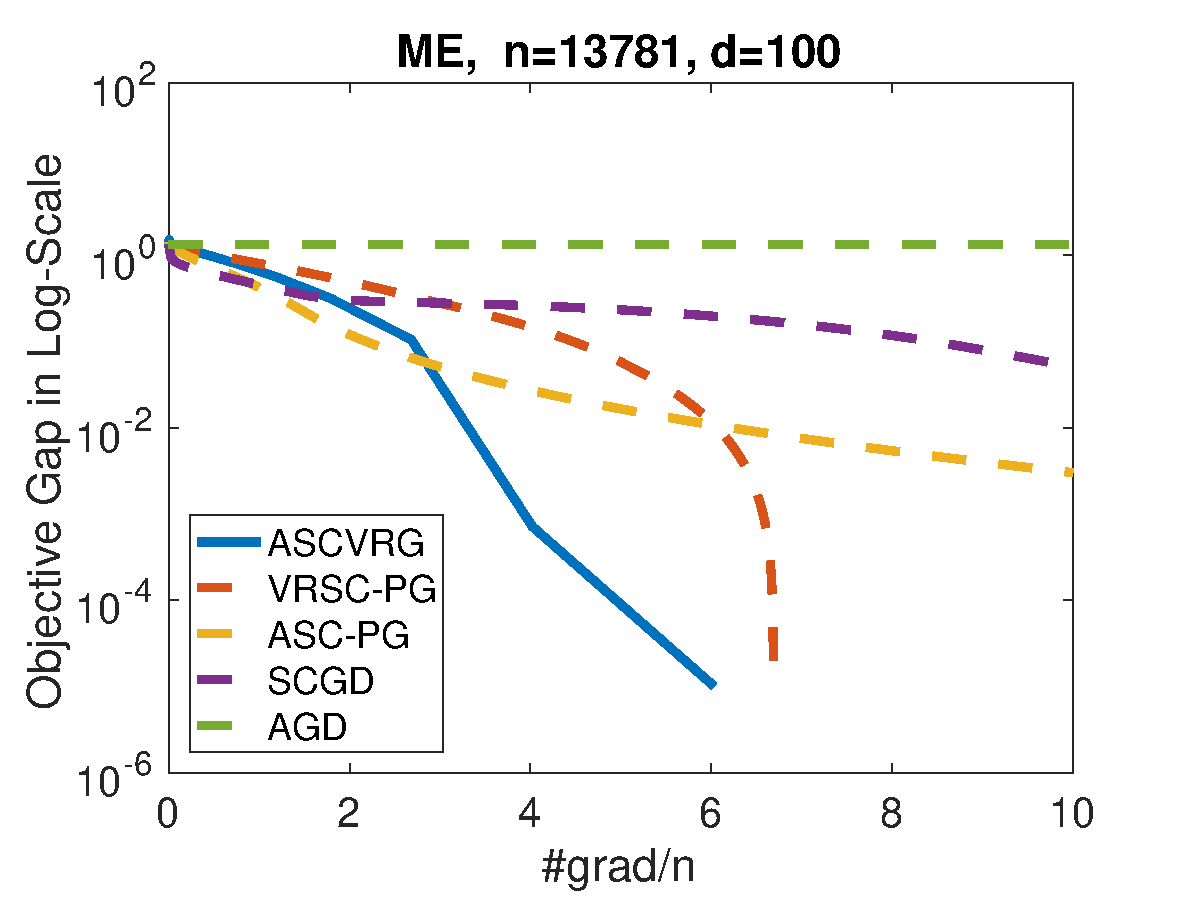
\includegraphics[width=0.38\textwidth]{figs/ME_All.eps}
}
\subfloat[Operating Profitability]{%
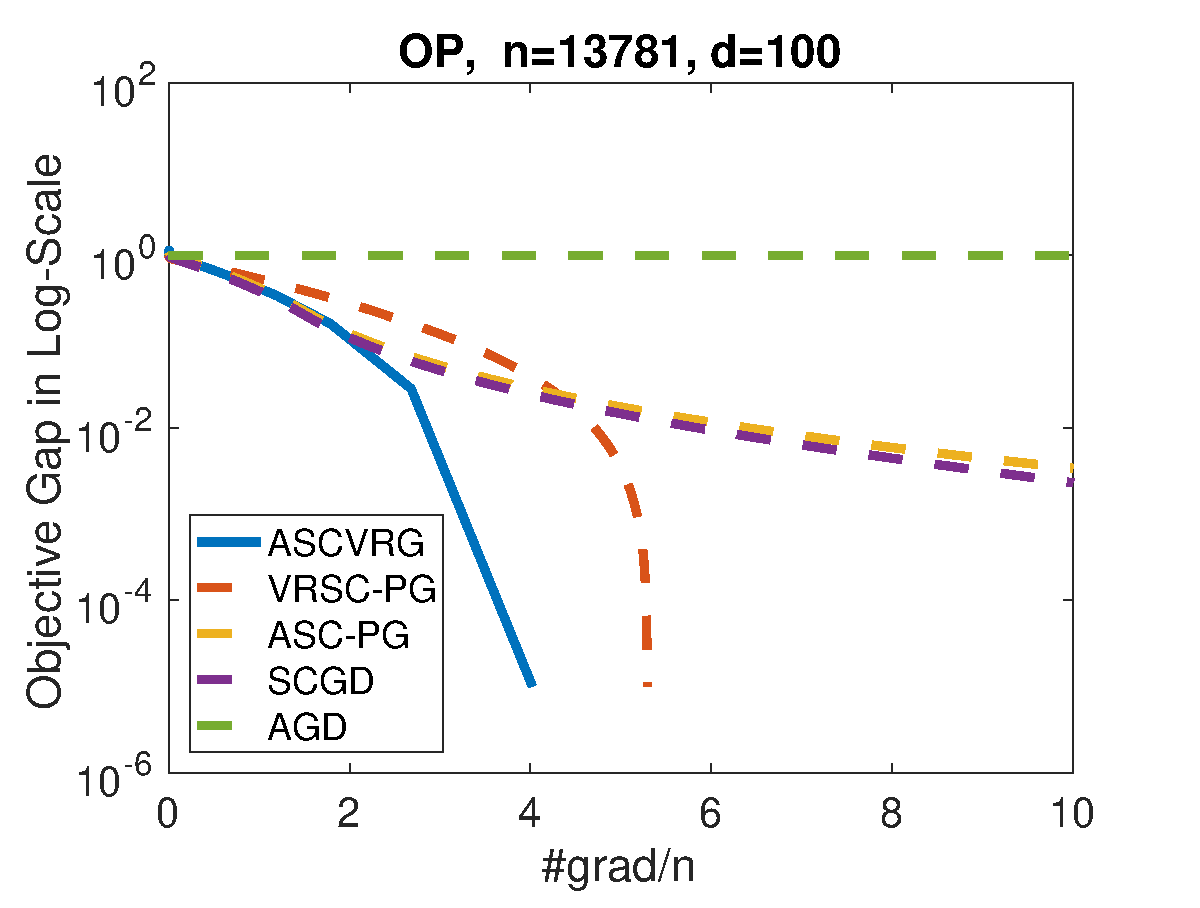
\includegraphics[width=0.38\textwidth]{figs/OP_All.eps}
}%
\subfloat[Investment]{%
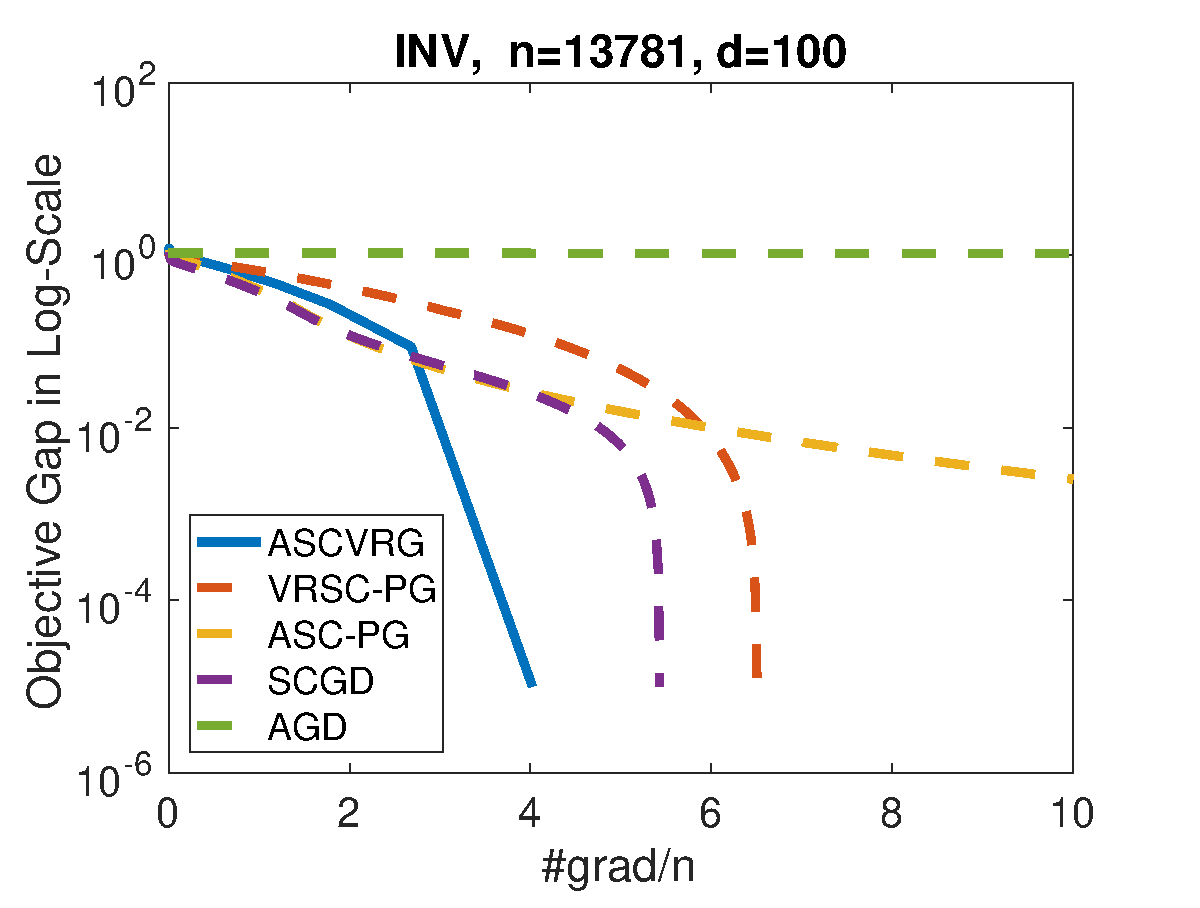
\includegraphics[width=0.38\textwidth]{figs/INV_All.eps}
}
\caption{The Performance of All Methods on three Large 100-Portfolio Datasets}\label{Fig:Large-Data}
\end{figure}

We set $\lambda=5\times10^{-7}$ in problem~\eqref{prob:SpMO} and $A=B=C=5$ and $\eta=1/2L_\phi$ in ASCVRG. For the $x$-axis, we use the number of gradient oracles divided by the number of samples, denoted as \#grad/n, which is proportional to the query complexity. For the $y$-axis, we use the log-scale of the objective gap $\Phi(\x)-\Phi(\x^*)$ where $\x^*$ is obtained by running ASCVRG for enough iterations until convergence and is used as the optimal solution for all methods.

Figure~\ref{Fig:Large-Data} shows that, on three large datasets, ASCVRG consistently outperforms the other four methods in terms of the IFO complexity. Moreover, ASCVRG and VRSC-PG are more robust than SCGD and ASC-PG, showing that the use of variance reduction together with constant step size stabilizes the behavior of the stochastic algorithms. Although SCGD and ASC-PG perform well on some datasets, pure stochastic gradient-type methods can be sensitive to choices of shrinking step sizes and thus require effort to tune parameters in practice \cite{Berahas-2017-Investigation}. In contrast, the step sizes of ASCVRG and VRSC-PG are not shrinking, yielding improved robustness in practice. As expected, AGD performs worse than other methods, having the highest IFO complexity on large datasets. 

Figures~\ref{Fig:Book_to_Market}-\ref{Fig:Investment} further show that, on 18 different medium datasets, ASCVRG consistently outperforms the other four methods in terms of the IFO complexity even if the margin is smaller than that on large datasets. Actually ASCVRG and VRSC-PG are comparable on nearly half of the datasets, significantly outperforming the other three methods by a large margin. This is consistent with the theoretical IFO complexity of ASCVRG and VRSC-PG. In comparison to ASCVRG's IFO complexity of $O\left((m+n)\log(1/\varepsilon)+1/\varepsilon^3\right)$, VRSC-PG's IFO complexity of $O(m+n+(m+n)^{2/3}/\varepsilon^2)$ is favorable when $m+n$ is not very large. On the other hand, we observe from Figures~\ref{Fig:Book_to_Market}-\ref{Fig:Investment} that VRSC-PG is less robust than ASCVRG. One possible reason is that VRSC-PG uses a constant step size while ASCVRG uses an adaptive but not shrinking step size. In sum, the ASCVRG method has the potential to be a benchmark algorithm for nonsmooth convex composition optimization. 

\section{Conclusions}\label{sec:conclusion}
We propose an accelerated stochastic compositional variance reduced gradient method for convex composition optimization. We establish a better IFO complexity than the best-known result prior to this paper under the same reasonable conditions. Experimental results on sparse mean-variance optimization with 21 real-world financial datasets demonstrate that our method outperforms other competing methods. An important direction for future work is to study the possibility of a lower oracle complexity for stochastic composition optimization and the optimal compositional gradient method. 
\begin{figure}[t] 
\hspace{-6em}
\subfloat[Asia{\_}Pacific{\_}ex{\_}Japan]{
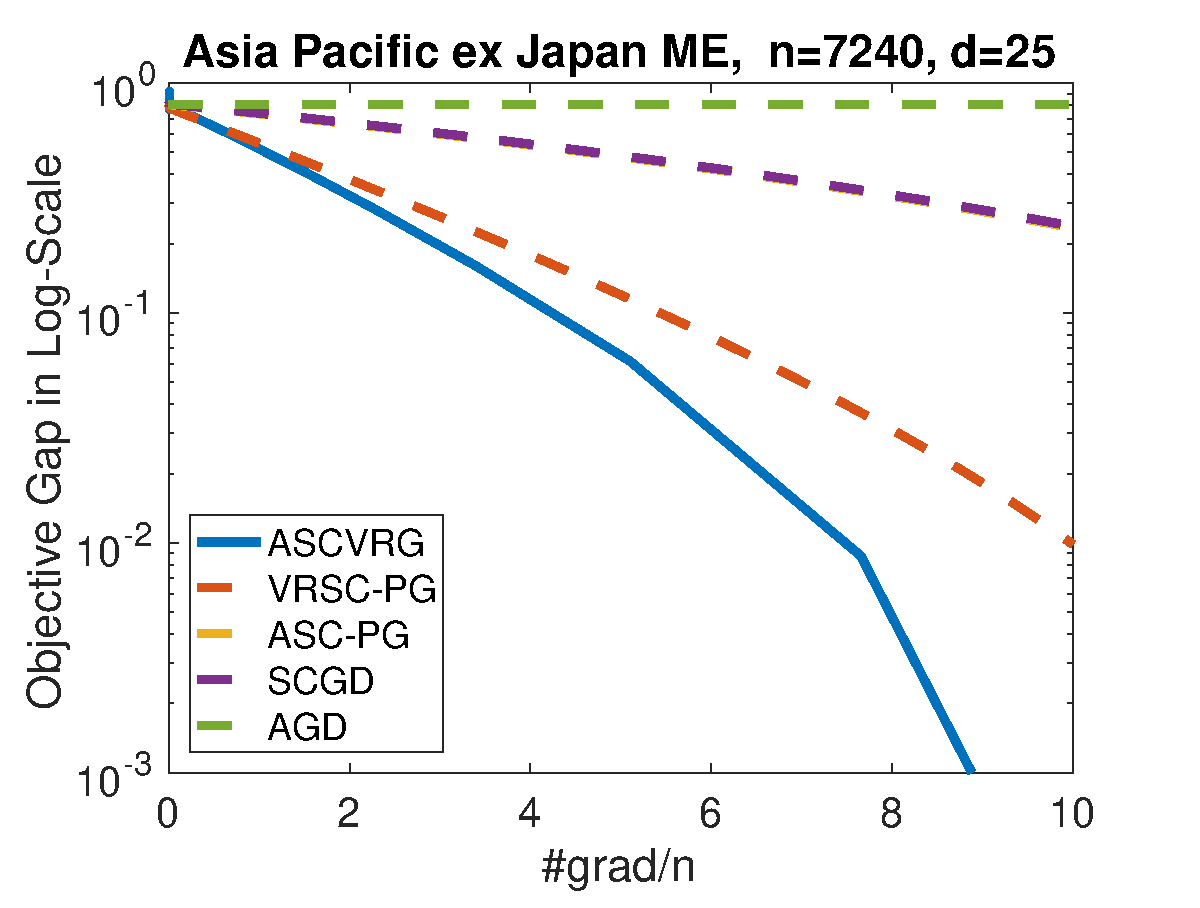
\includegraphics[width=0.2\textwidth]{figs/ME_Asia_Pacific_ex_Japan.eps}%
}
\subfloat[Europe]{%
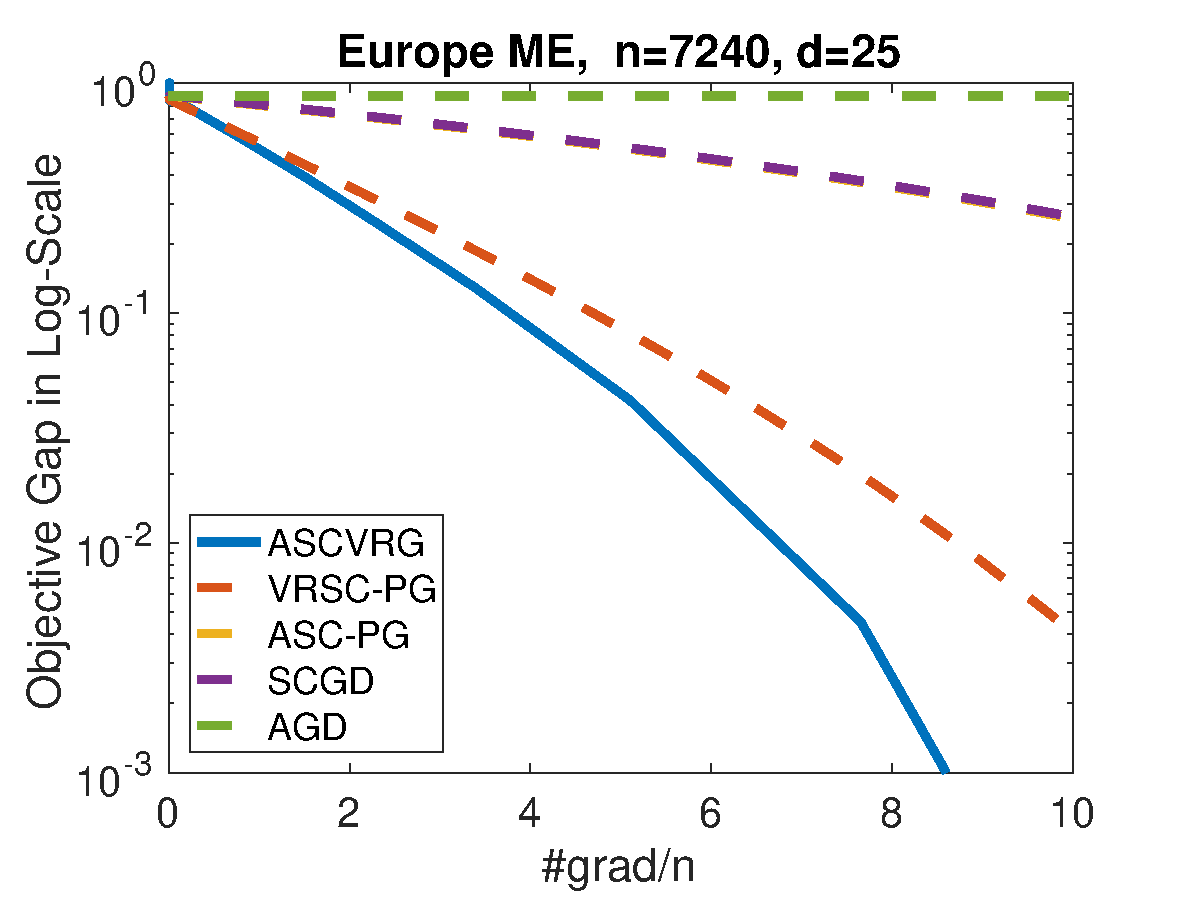
\includegraphics[width=0.2\textwidth]{figs/ME_Europe.eps}%
}%
\subfloat[Global{\_}ex{\_}US]{%
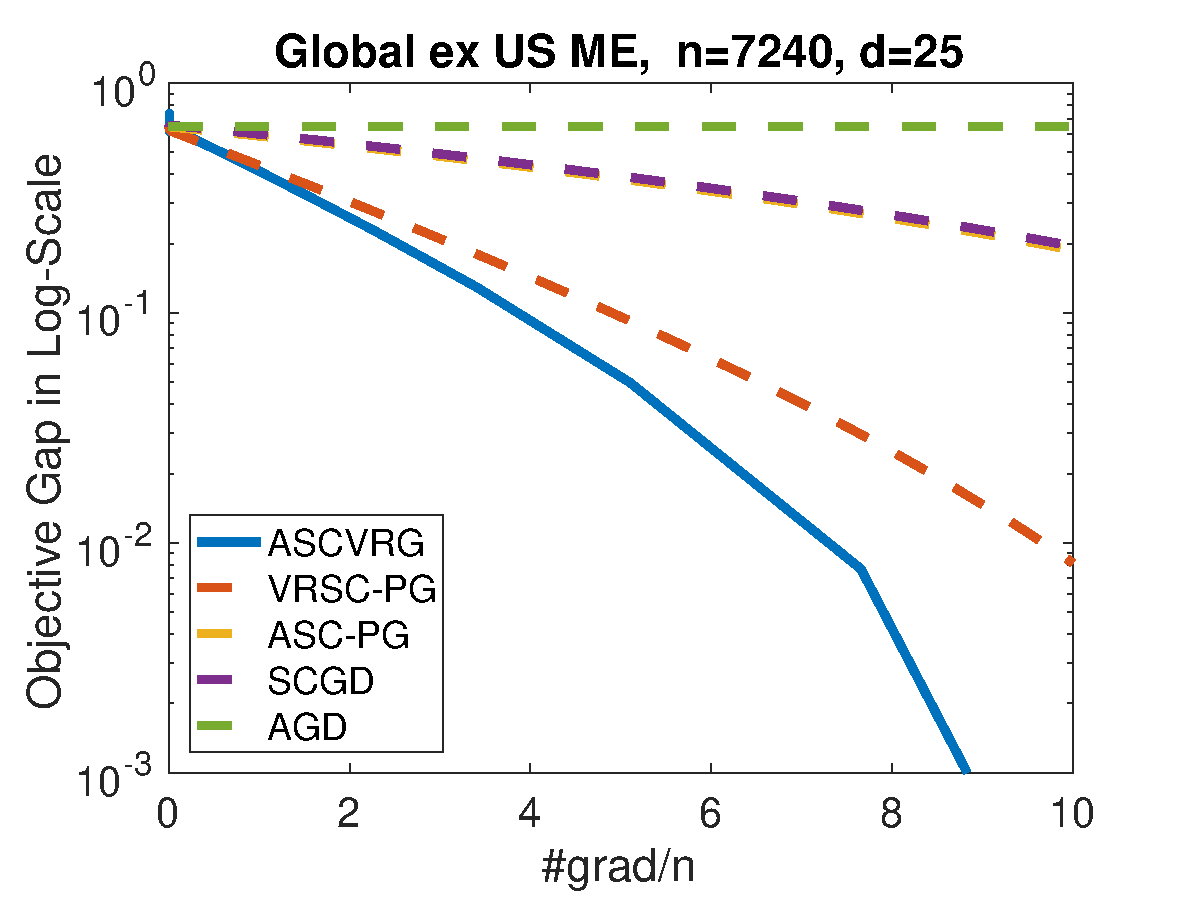
\includegraphics[width=0.2\textwidth]{figs/ME_Global_ex_US.eps}%
}%
\subfloat[Global]{%
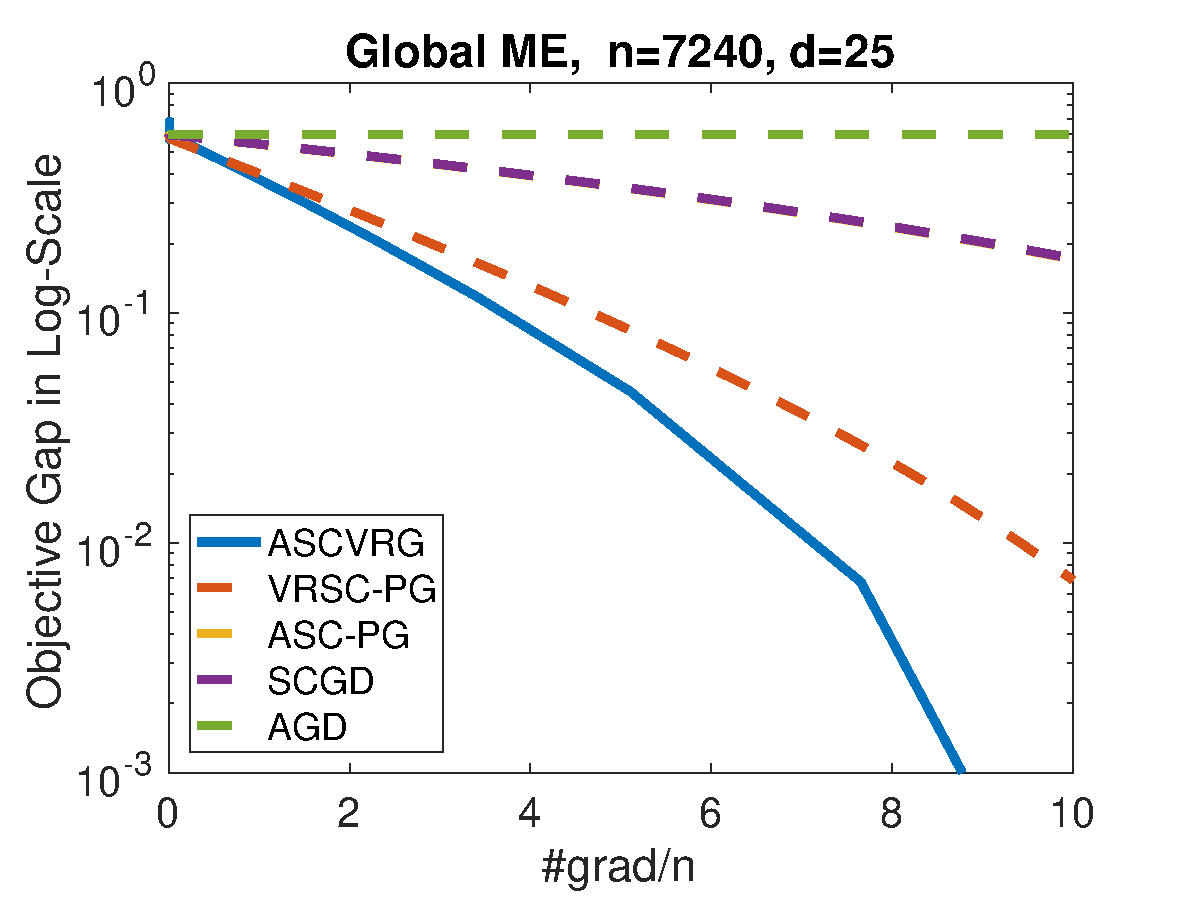
\includegraphics[width=0.2\textwidth]{figs/ME_Global.eps}%
}%
\subfloat[Japan]{%
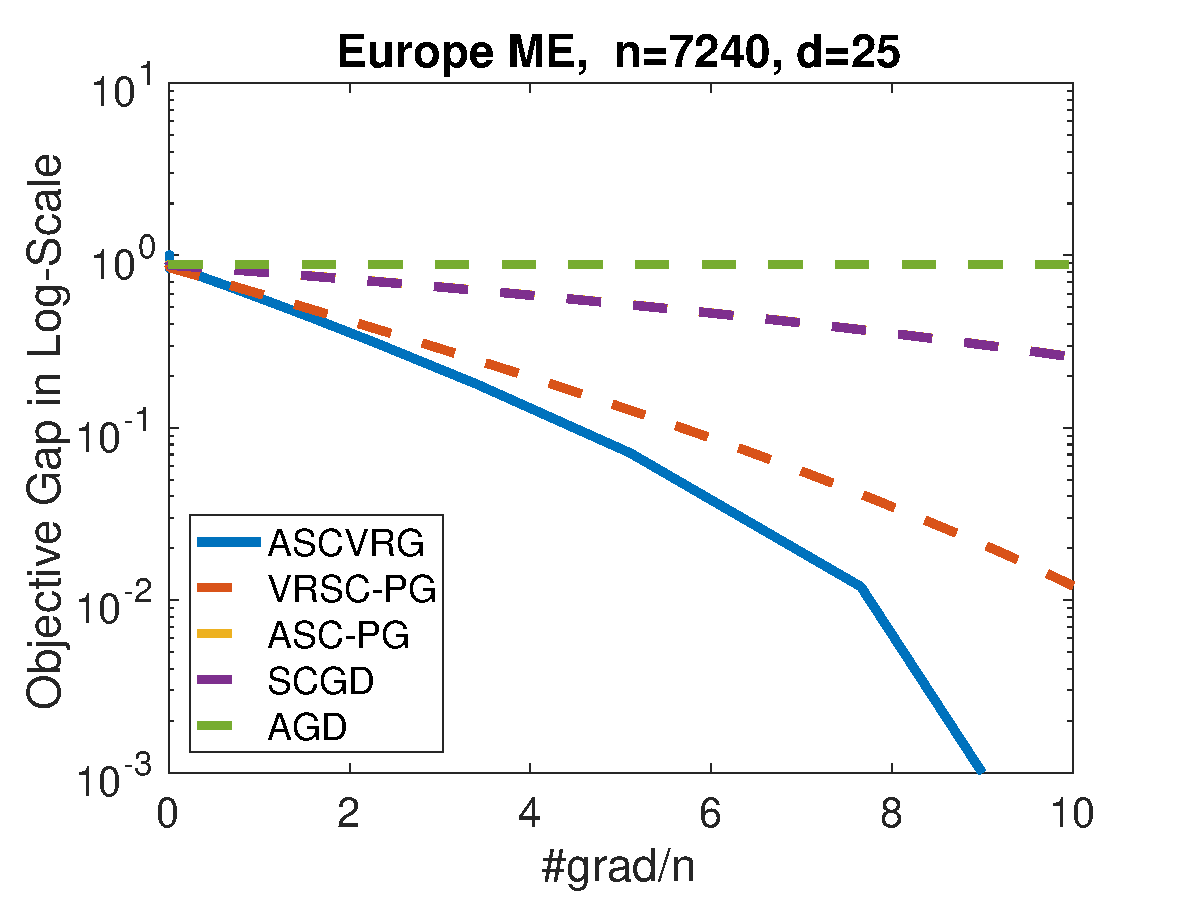
\includegraphics[width=0.2\textwidth]{figs/ME_Japan.eps}%
}%
\subfloat[North{\_}America]{%
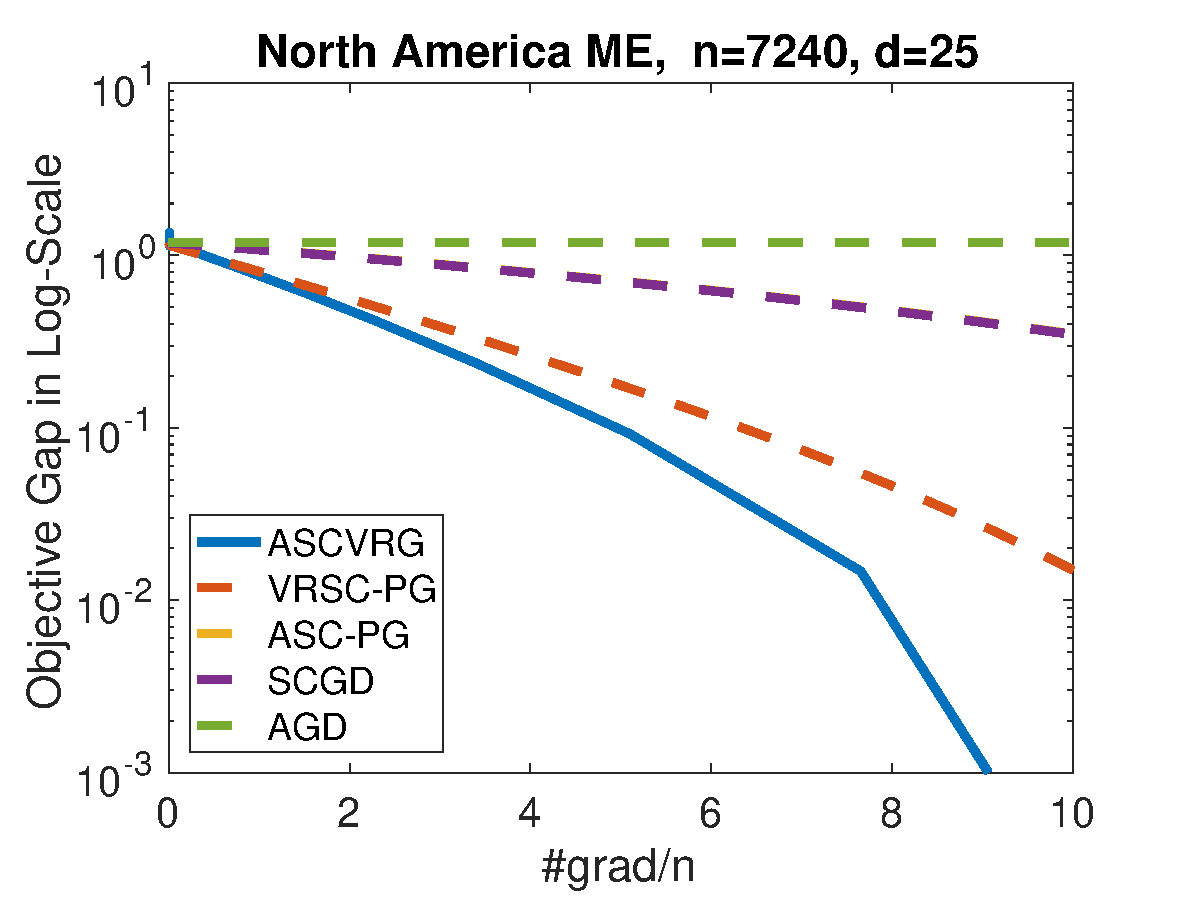
\includegraphics[width=0.2\textwidth]{figs/ME_North_America.eps}%
}%
\caption{The Performance of All Methods on six 25-Portfolio Book-to-Market Datasets} \label{Fig:Book_to_Market}
\end{figure}

\begin{figure}[t] 
\hspace{-6em}
\subfloat[Asia{\_}Pacific{\_}ex{\_}Japan]{
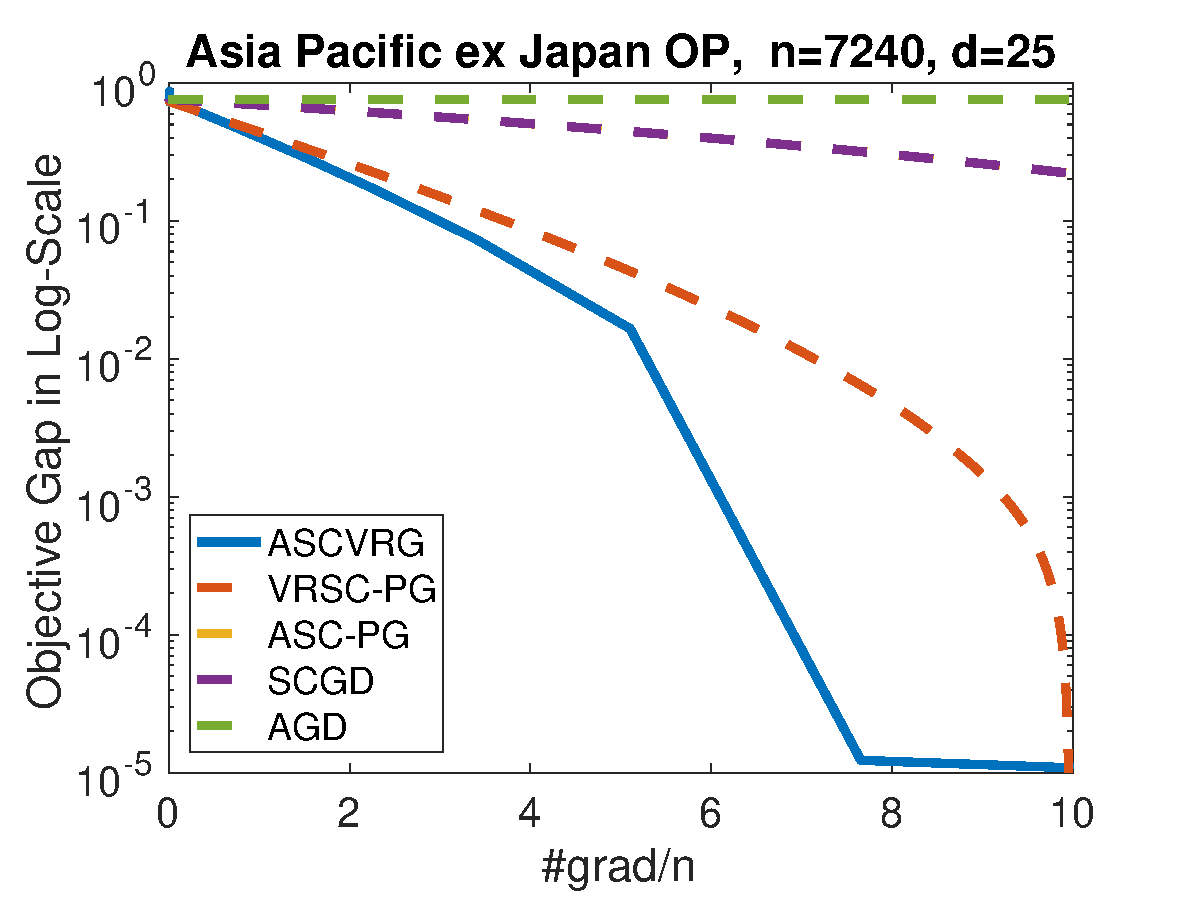
\includegraphics[width=0.2\textwidth]{figs/OP_Asia_Pacific_ex_Japan.eps}%
}
\subfloat[Europe]{%
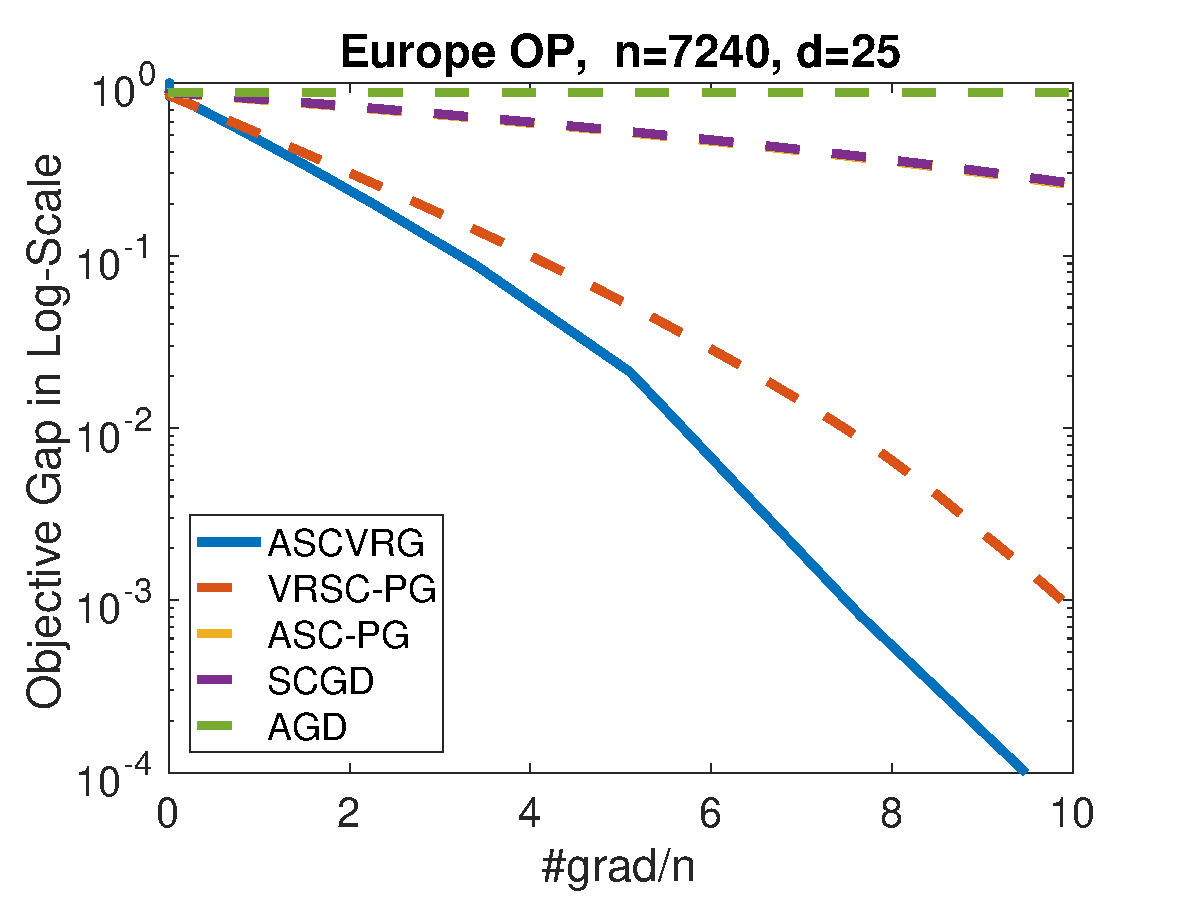
\includegraphics[width=0.2\textwidth]{figs/OP_Europe.eps}%
}%
\subfloat[Global{\_}ex{\_}US]{%
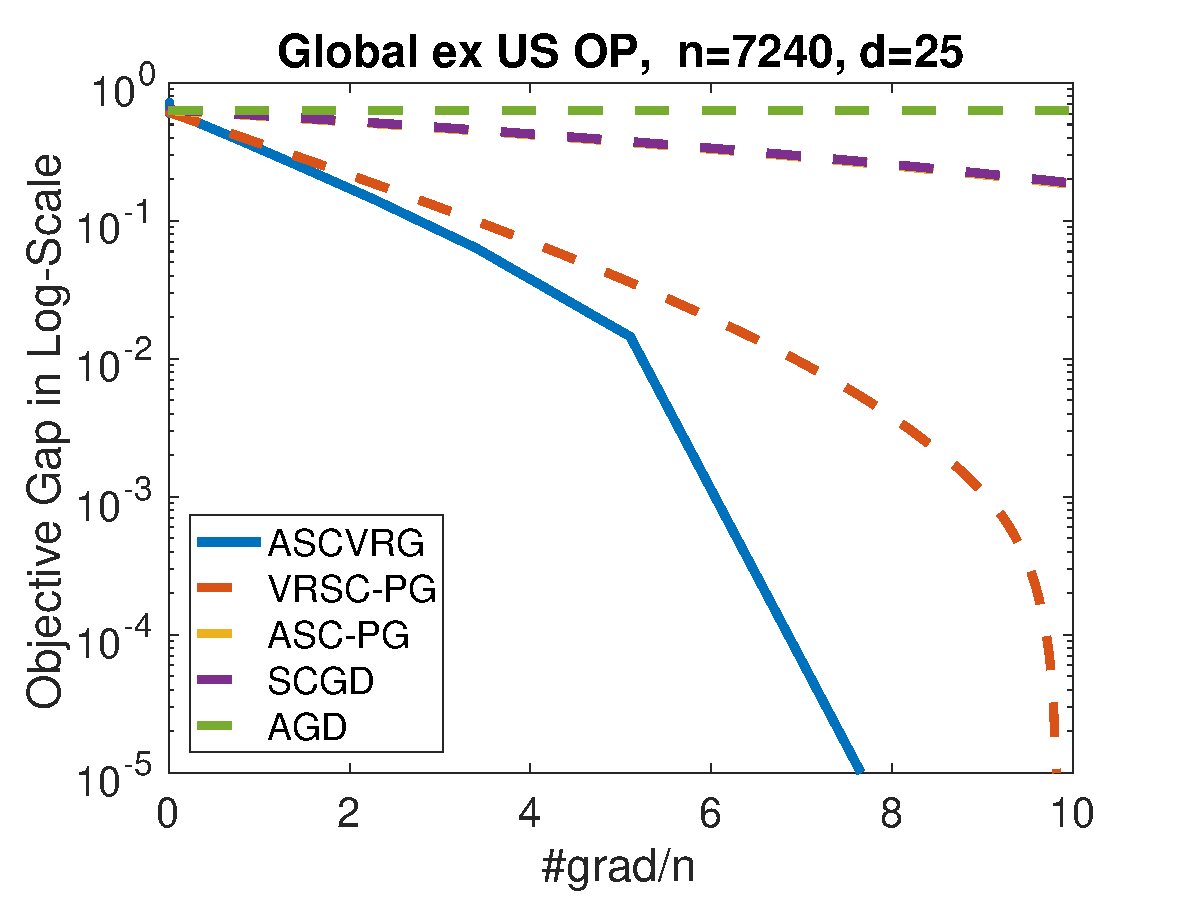
\includegraphics[width=0.2\textwidth]{figs/OP_Global_ex_US.eps}%
}%
\subfloat[Global]{%
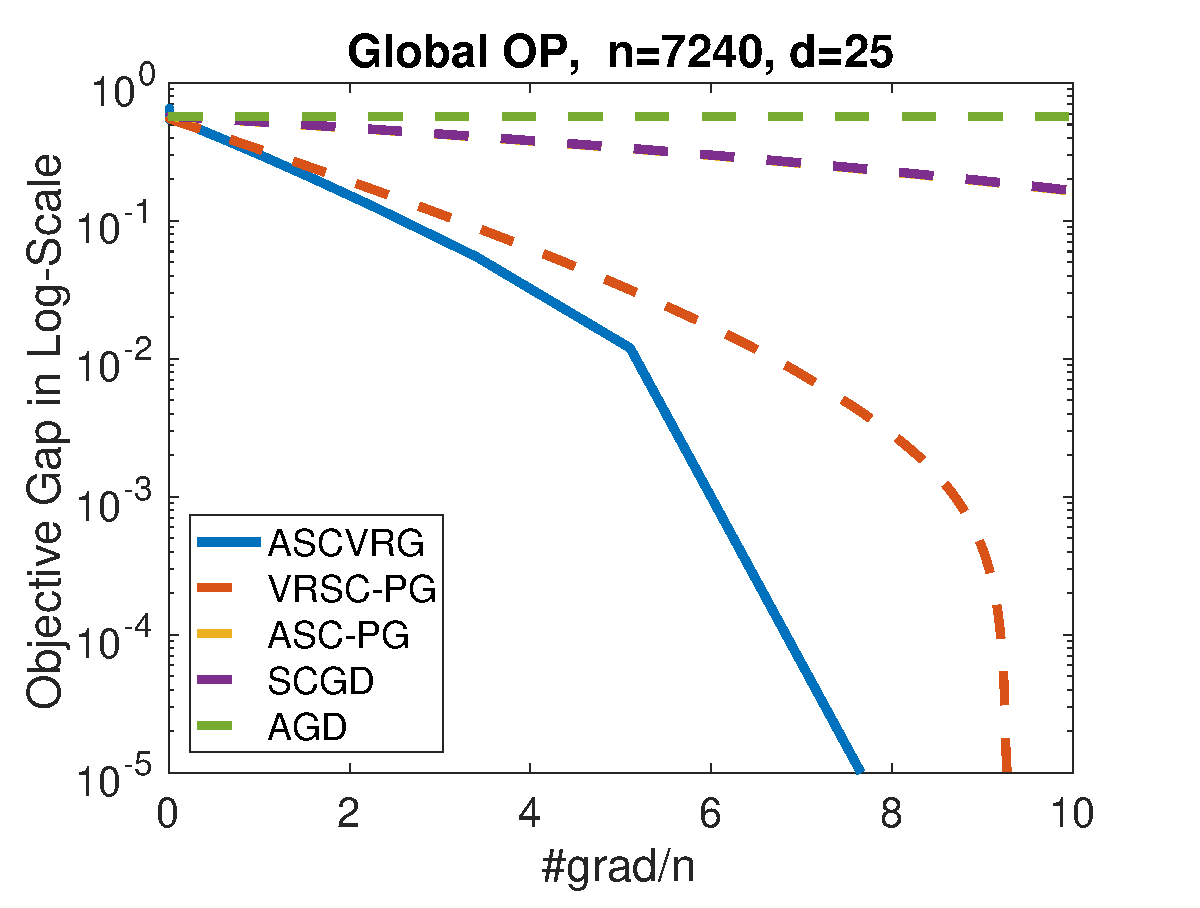
\includegraphics[width=0.2\textwidth]{figs/OP_Global.eps}%
}%
\subfloat[Japan]{%
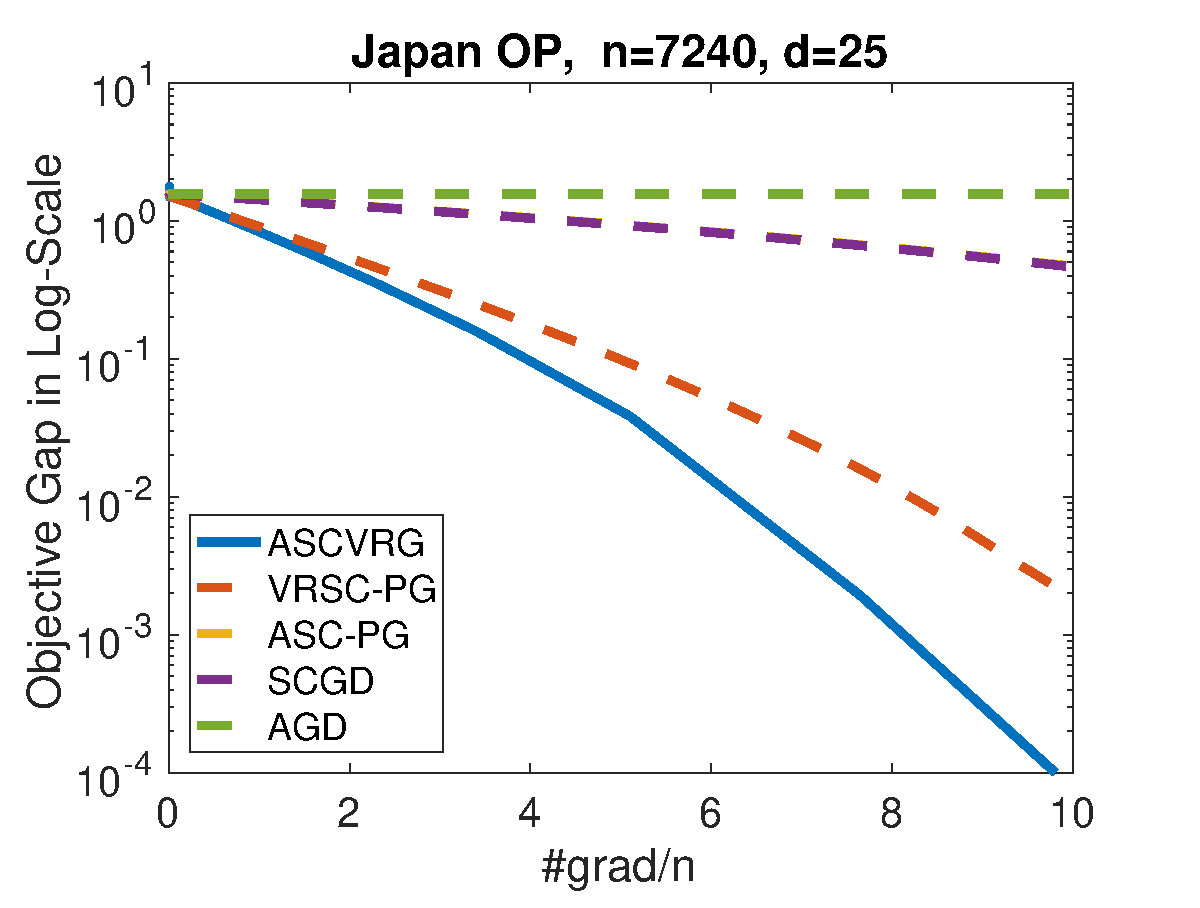
\includegraphics[width=0.2\textwidth]{figs/OP_Japan.eps}%
}%
\subfloat[North{\_}America]{%
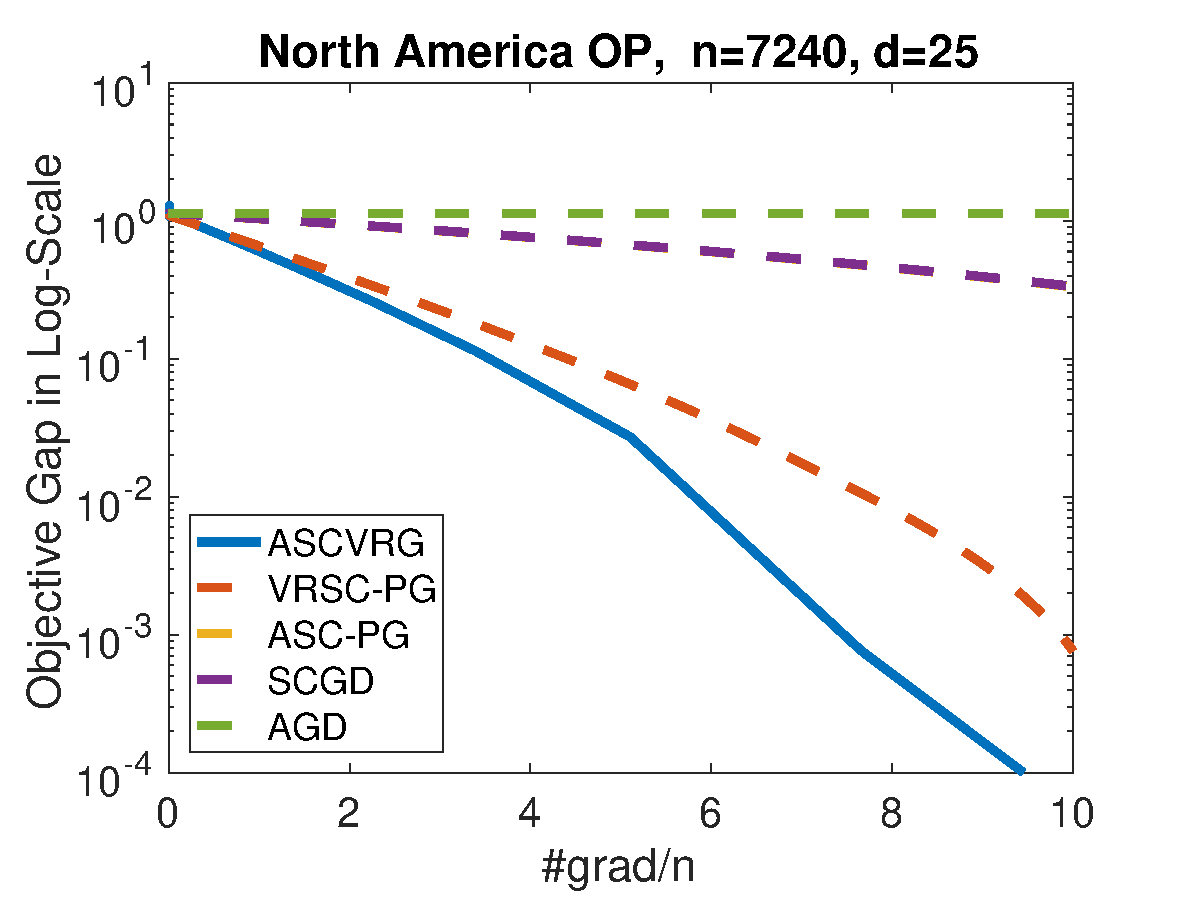
\includegraphics[width=0.2\textwidth]{figs/OP_North_America.eps}%
}%
\caption{The Performance of All Methods on six 25-Portfolio Operating Profitability Datasets} \label{Fig:Operating_Profitability}
\end{figure}

\begin{figure}[!t]
\hspace{-6em}
\subfloat[Asia{\_}Pacific{\_}ex{\_}Japan]{
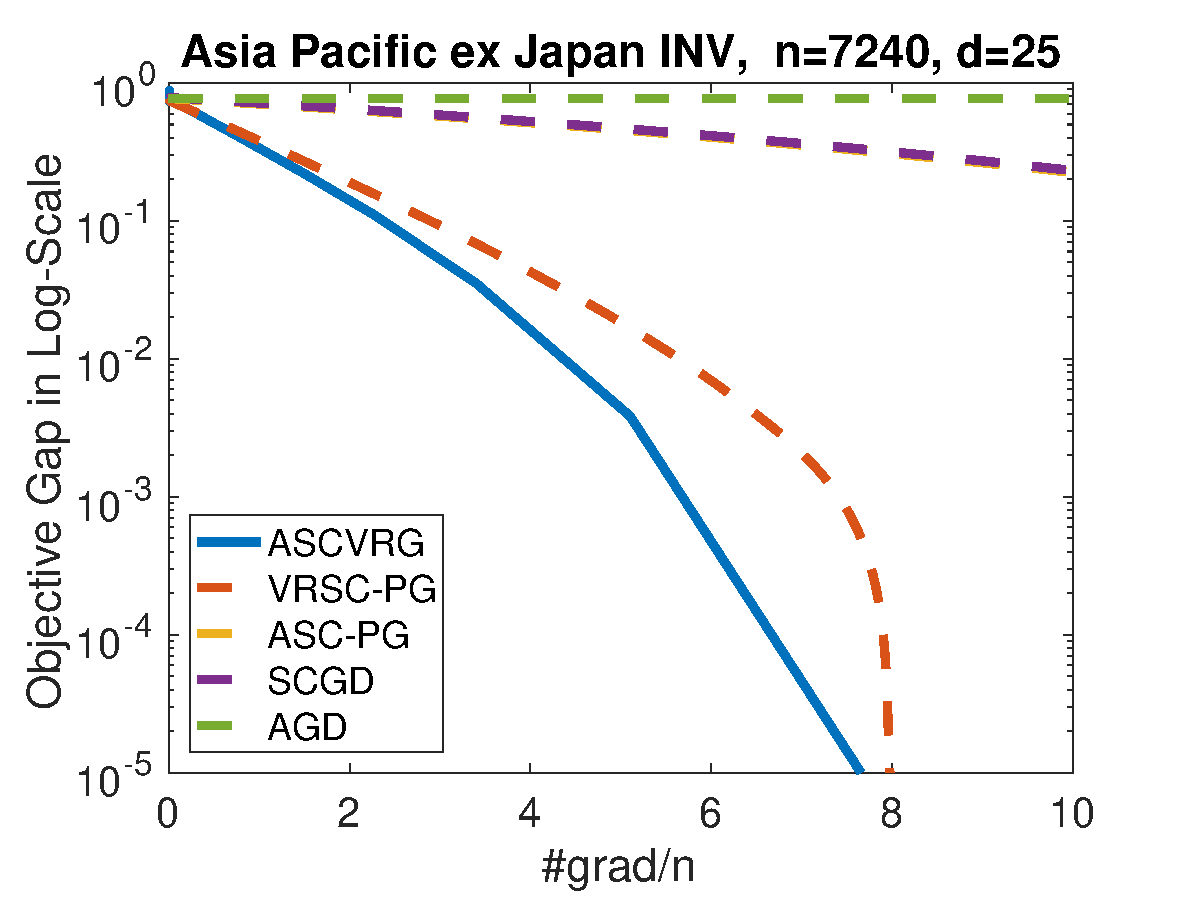
\includegraphics[width=0.2\textwidth]{figs/INV_Asia_Pacific_ex_Japan.eps}%
}
\subfloat[Europe]{%
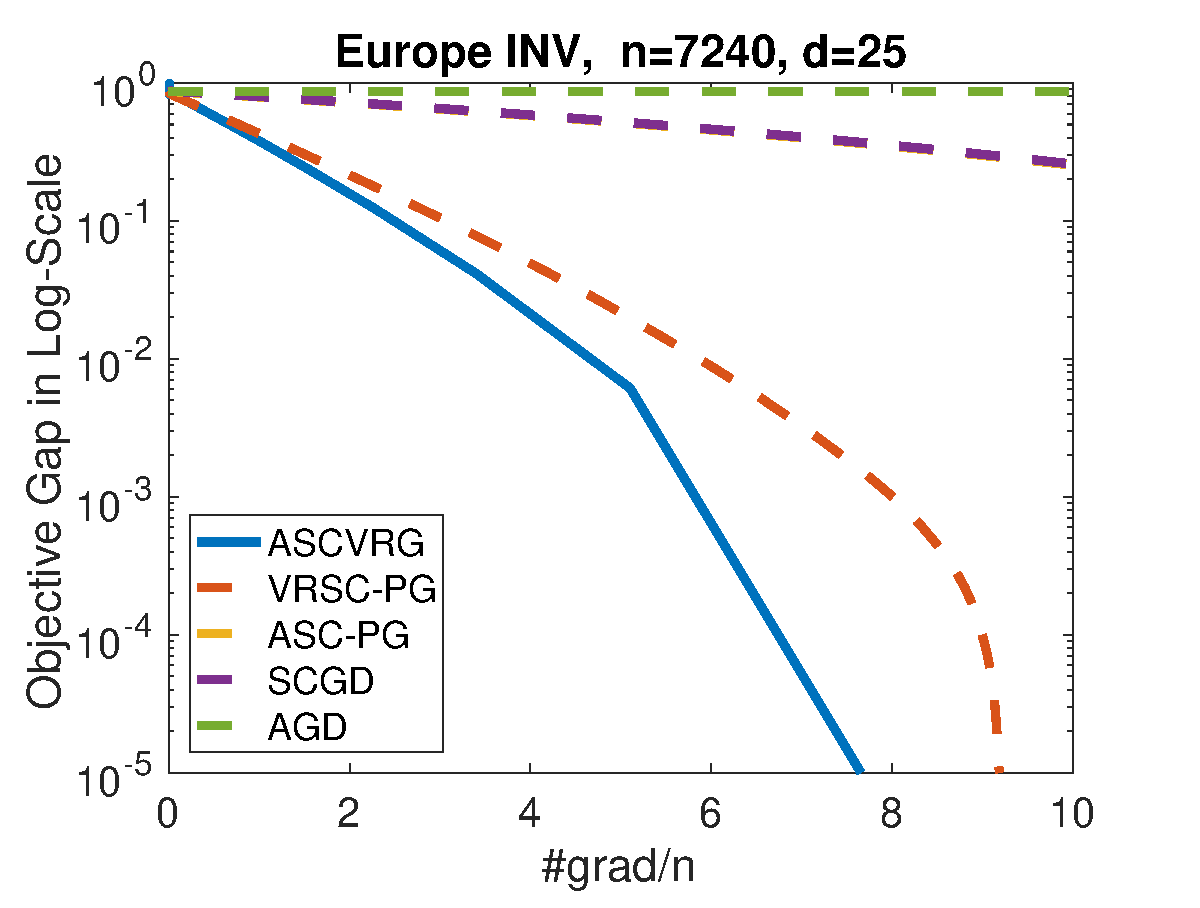
\includegraphics[width=0.2\textwidth]{figs/INV_Europe.eps}%
}%
\subfloat[Global{\_}ex{\_}US]{%
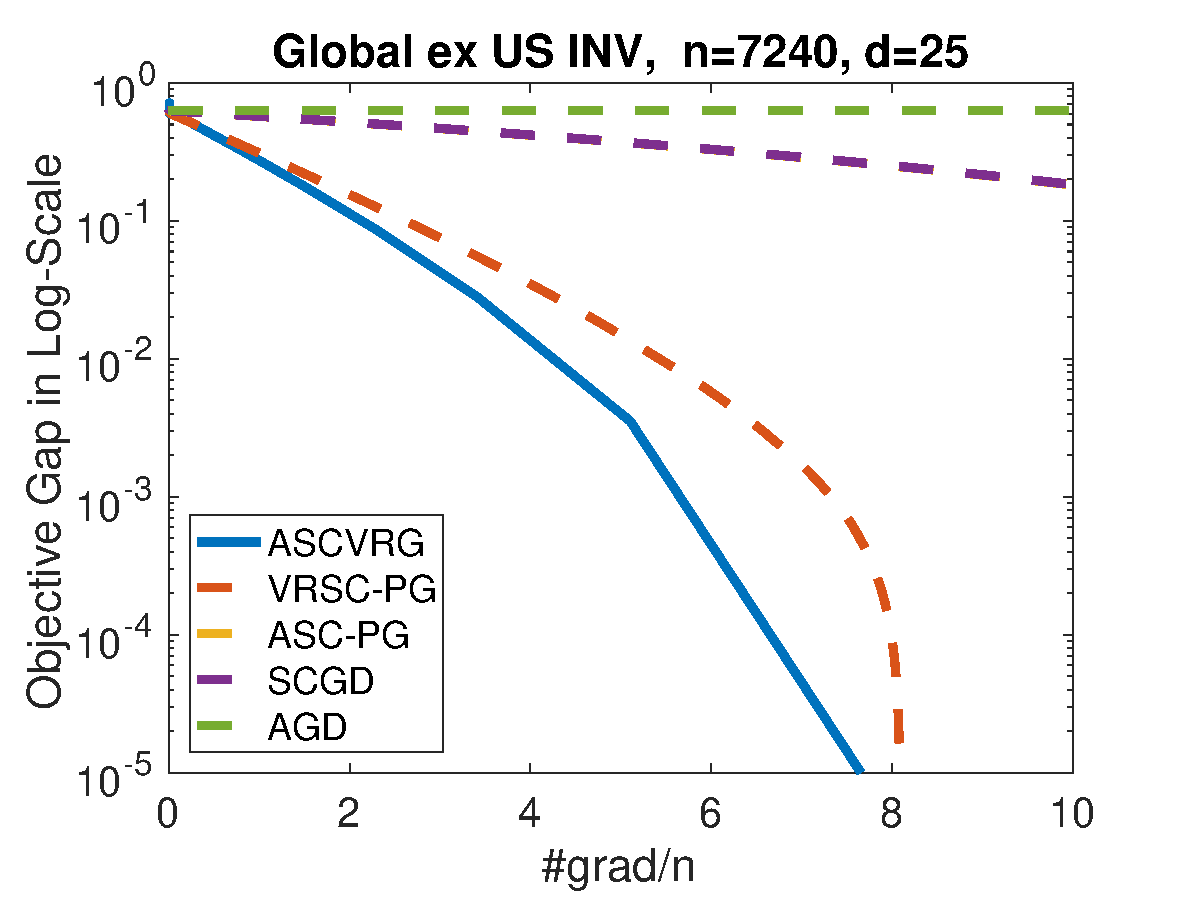
\includegraphics[width=0.2\textwidth]{figs/INV_Global_ex_US.eps}%
}%
\subfloat[Global]{%
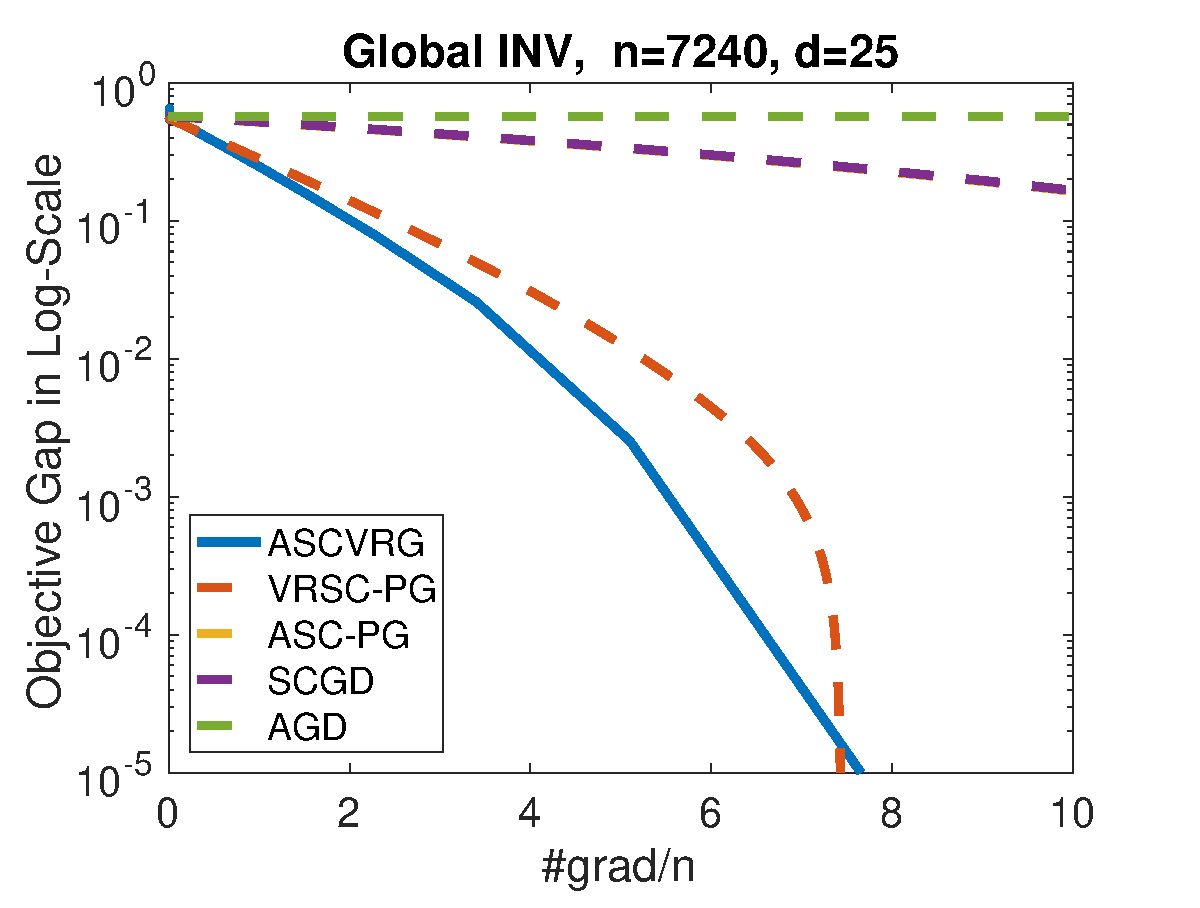
\includegraphics[width=0.2\textwidth]{figs/INV_Global.eps}%
}%
\subfloat[Japan]{%
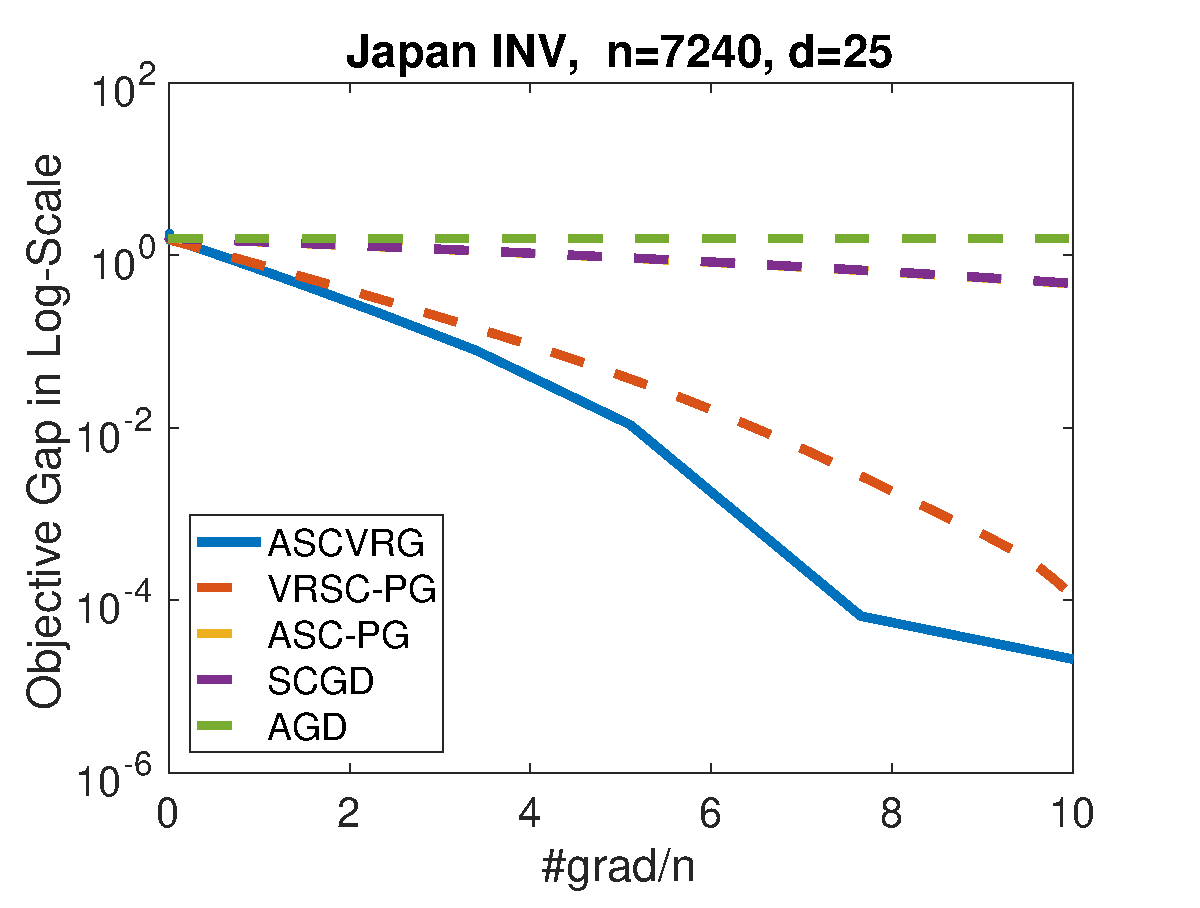
\includegraphics[width=0.2\textwidth]{figs/INV_Japan.eps}%
}%
\subfloat[North{\_}America]{%
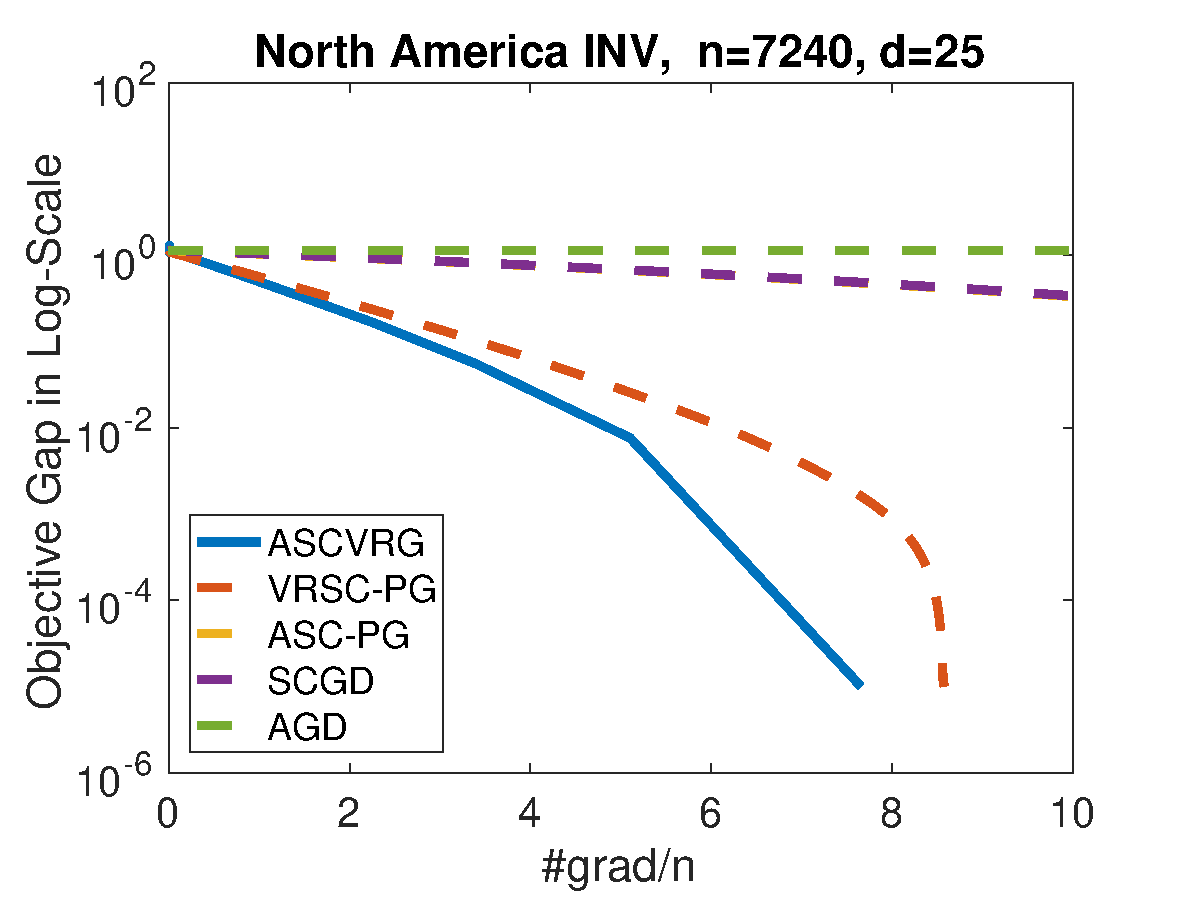
\includegraphics[width=0.2\textwidth]{figs/INV_North_America.eps}%
}%
\caption{The Performance of All Methods on six 25-Portfolio Investment Datasets} \label{Fig:Investment}
\end{figure}

\begin{thebibliography}{10}
\bibitem{Agarwal-2015-Lower}
A.~Agarwal and L.~Bottou.
\newblock A lower bound for the optimization of finite sums.
\newblock In {\em ICML}, pages 78--86, 2015.

\bibitem{Allen-2017-Natasha}
Z.~Allen-Zhu.
\newblock Natasha: Faster non-convex stochastic optimization via strongly non-convex parameter.
\newblock In {\em ICML}, pages 89--97, 2017.

\bibitem{Allen-2016-Variance}
Z.~Allen-Zhu and E.~Hazan.
\newblock Variance reduction for faster non-convex optimization.
\newblock In {\em ICML}, pages 699--707, 2016.

\bibitem{Allen-2016-Improved}
Z.~Allen-Zhu and Y.~Yuan.
\newblock Improved {SVRG} for non-strongly-convex or sum-of-non-convex objectives.
\newblock In {\em ICML}, pages 1080--1089, 2016.

\bibitem{Berahas-2017-Investigation}
A.~S. Berahas, R.~Bollapragada, and J.~Nocedal.
\newblock An investigation of {N}ewton-sketch and subsampled {N}ewton methods.
\newblock {\em ArXiv Preprint: 1705.06211}, 2017.

\bibitem{Goodfellow-2016-Deep}
I.~Goodfellow, Y.~Bengio, and A.~Courville.
\newblock {\em Deep Learning}.
\newblock MIT press, 2016.

\bibitem{Hu-2015-Model}
J.~Hu.
\newblock Model-based stochastic search methods.
\newblock In {\em Handbook of Simulation Optimization}, pages 319--340. Springer, 2015.

\bibitem{Huang-2010-Variable}
J.~Huang, J.~L. Horowitz, and F.~Wei.
\newblock Variable selection in nonparametric additive models.
\newblock {\em Annals of Statistics}, 38(4):2282, 2010.

\bibitem{Huo-2017-Accelerated}
Z.~Huo, B.~Gu, and H.~Huang.
\newblock Accelerated method for stochastic composition optimization with nonsmooth regularization.
\newblock {\em ArXiv Preprint: 1711.03937}, 2017.

\bibitem{Johnson-2013-Accelerating}
R.~Johnson and T.~Zhang.
\newblock Accelerating stochastic gradient descent using predictive variance reduction.
\newblock In {\em NIPS}, pages 315--323, 2013.

\bibitem{Kundur-1994-Power}
P.~Kundur, N.~J. Balu, and M.~G. Lauby.
\newblock {\em Power System Stability and Control}, volume~7.
\newblock McGraw-hill New York, 1994.

\bibitem{Lei-2017-Nonconvex}
L.~Lei, C.~Ju, J.~Chen, and M.~I. Jordan.
\newblock Nonconvex finite-sum optimization via {SCSG} methods.
\newblock {\em ArXiv Preprint: 1706.09156}, 2017.

\bibitem{Lian-2017-Finite}
X.~Lian, M.~Wang, and J.~Liu.
\newblock Finite-sum composition optimization via variance reduced gradient descent.
\newblock In {\em AISTATS}, pages 1159--1167, 2017.

\bibitem{Nesterov-2013-Introductory}
Y.~Nesterov.
\newblock {\em Introductory Lectures on Convex Optimization: A Basic Course}, volume~87.
\newblock Springer Science \& Business Media, 2013.

\bibitem{Puterman-2014-Markov}
M.~L. Puterman.
\newblock {\em Markov Decision Processes: Discrete Stochastic Dynamic Programming}.
\newblock John Wiley \& Sons, 2014.

\bibitem{Ravikumar-2009-Sparse}
P.~Ravikumar, J.~Lafferty, H.~Liu, and L.~Wasserman.
\newblock Sparse additive models.
\newblock {\em Journal of the Royal Statistical Society. Series B, Statistical Methodology}, pages 1009--1030, 2009.

\bibitem{Reddi-2016-Stochastic}
S.~J. Reddi, A.~Hefny, S.~Sra, B.~Poczos, and A.~Smola.
\newblock Stochastic variance reduction for nonconvex optimization.
\newblock In {\em ICML}, pages 314--323, 2016.

\bibitem{Rockafellar-2000-Optimization}
R.~T. Rockafellar and S.~Uryasev.
\newblock Optimization of conditional value-at-risk.
\newblock {\em Journal of Risk}, 2:21--42, 2000.

\bibitem{Schmidt-2017-Minimizing}
M.~Schmidt, N.~Le~Roux, and F.~Bach.
\newblock Minimizing finite sums with the stochastic average gradient.
\newblock {\em Mathematical Programming}, 162(1-2):83--112, 2017.

\bibitem{Shalev-2012-Online}
S.~Shalev-Shwartz.
\newblock Online learning and online convex optimization.
\newblock {\em Foundations and Trends{\textregistered} in Machine Learning}, 4(2):107--194, 2012.

\bibitem{Shalev-2016-SDCA}
S.~Shalev-Shwartz.
\newblock {SDCA} without duality, regularization, and individual convexity.
\newblock In {\em ICML}, pages 747--754, 2016.

\bibitem{Shalev-2013-Stochastic}
S.~Shalev-Shwartz and T.~Zhang.
\newblock Stochastic dual coordinate ascent methods for regularized loss minimization.
\newblock {\em Journal of Machine Learning Research}, 14(Feb):567--599, 2013.

\bibitem{Shamir-2016-Fast}
O.~Shamir.
\newblock Fast stochastic algorithms for {SVD} and {PCA}: Convergence properties and convexity.
\newblock In {\em ICML}, pages 248--256, 2016.

\bibitem{Shapiro-2009-Lectures}
A.~Shapiro, D.~Dentcheva, and A.~Ruszczy{\'n}ski.
\newblock {\em Lectures on Stochastic Programming: Modeling and Theory}.
\newblock SIAM, 2009.

\bibitem{Sutton-1998-Reinforcement}
R.~S. Sutton and A.~G. Barto.
\newblock {\em Reinforcement Learning: An Introduction}, volume~1.
\newblock MIT press Cambridge, 1998.

\bibitem{Wang-2017-Stochastic}
M.~Wang, E.~X. Fang, and H.~Liu.
\newblock Stochastic compositional gradient descent: algorithms for minimizing compositions of expected-value functions.
\newblock {\em Mathematical Programming}, 161(1-2):419--449, 2017.

\bibitem{Wang-2017-Accelerating}
M.~Wang, J.~Liu, and E.~X. Fang.
\newblock Accelerating stochastic composition optimization.
\newblock {\em Journal of Machine Learning Research}, 18:1--23, 2017.

\bibitem{Woodworth-2016-Tight}
B.~E. Woodworth and N.~Srebro.
\newblock Tight complexity bounds for optimizing composite objectives.
\newblock In {\em NIPS}, pages 3639--3647, 2016.

\bibitem{Yang-2018-Multi}
S.~Yang, M.~Wang, and E.~X. Fang.
\newblock Multi-level stochastic gradient methods for nested compositon optimization.
\newblock {\em ArXiv Preprint: 1801.03600}, 2018.

\bibitem{Yu-2017-Fast}
Y.~Yu and L.~Huang.
\newblock Fast stochastic variance reduced {ADMM} for stochastic composition optimization.
\newblock {\em ArXiv Preprint: 1705.04138}, 2017.
\end{thebibliography}

\appendix
\section{Proof Outline}
We list the assumptions in our paper and some major steps to give a whole picture of the proof. 
\begin{center}
\shadowbox{\begin{minipage}{6in}
\textbf{Proof Outlines:}
\begin{enumerate}
\item We provide two basic lemmas, which concerns with convex objective and common variance; see Lemmas~\ref{Lemma:SampleGradient-Variance} and~\ref{Lemma:Gradient-Objective}. 
\item We bound the term of $\BE\left[\left\| \sv_t^{s+1} - \nabla f(\x_t^{s+1}) \right\|^2 \mid \x_t^{s+1}, \tilde{\x}^s\right]$ using the term $\left\|\tilde{\x}^s - \x^*\right\|^2$, $\left\| \x_t^{s+1} - \x^*\right\|^2$ and the size of $\ACal_t$, $\BCal_t$ and $\CCal_t$, i.e., $A$, $B$ and $C$; see Lemma~\ref{Lemma:Gradient-Variance}. 
\item We bound the term of $\BE\left[\Phi(\tilde{\x}^{s+1}) \right] - \Phi(\x^*) $ using the term $\Phi(\x^0) - \Phi(\x^*)$, $\left\| \x^0 - \x^*\right\|^2$ and the parameters $\eta$ and $k_0$; see Lemmas~\ref{Lemma:Objective-Variational-Inequality} and \ref{Lemma:Objective-Gap}. 
\item We provide the explicit IFO complexity in terms of $m+n$, $L_\phi$, $L_f$, $L_g$, $B_f$ and $B_g$; see Theorem~\ref{Theorem:Main}. 
\end{enumerate}
\end{minipage}}
\end{center}
\begin{assumption}\label{Assumption:Objective-Convex}
The objective $F$ and $r$ are both convex, i.e., 
\begin{eqnarray*}
F(\x) - F(\y) - \left\langle \nabla F(\y), \x-\y\right\rangle & \geq & 0, \quad \x, \y \in \br^d, \\ 
r(\x) - r(\y) - \left\langle\xi, \x-\y\right\rangle & \geq & 0, \quad \x, \y \in \br^d, 
\end{eqnarray*}
where $\xi\in\partial r(\y)$ is a subgradient of $r$.  
\end{assumption}
\begin{assumption}
The proximal mapping of the objective $r$, given by
\begin{eqnarray*}
\argmin_{\x\in\br^d}\left\{ \left\langle \g, \x\right\rangle + \frac{1}{2\eta}\left\| \x - \y\right\|^2 + r(\x)\right\}, 
\end{eqnarray*}
is easily computed for any given $\g\in\br^d$ and $\y\in\br^d$ and $\eta>0$. 
\end{assumption}
\begin{assumption}\label{Assumption:Smooth-Gradient-Jacobian}
For $i\in[n]$ and $j\in[m]$, there exist constants $0<L_f, L_g, L_{\phi}<\infty$ such that
\begin{eqnarray*}
\left\| \nabla f_i(\x) - \nabla f_i(\y)\right\| & \leq & L_f \left\|\x-\y\right\|, \quad \x, \y \in \br^l, \\
\left\| \partial g_j(\x) - \partial g_j(\y)\right\| & \leq & L_g \left\|\x-\y\right\|, \quad \x, \y \in \br^d,
\end{eqnarray*}
and
\begin{equation*}
\left\| \left[\partial g_j(\x)\right]^\top \nabla f_i(g(\x))- \left[\partial g_j(\y)\right]^\top \nabla f_i(g(\y))\right\| \leq L_{\phi}\left\|\x-\y\right\|, \quad \x, \y \in \br^d. 
\end{equation*}
\end{assumption}
Intuitively, the constants $L_f$, $L_g$ and $L_\phi$ jointly characterize the smoothness and complexity of stochastic composition optimization. 
\begin{assumption}\label{Assumption:Bound-Jacobian-Gradient}
For $i\in[n]$ and $j\in[m]$, there exist two constants $0 < B_f, B_g < \infty$ such that
\begin{equation*}
\left\| \partial g_j(\x) \right\| \leq B_g, \ \x\in\br^d, \qquad \left\| \nabla f_i(\x) \right\| \leq B_f, \ \x \in \br^l. 
\end{equation*}
\end{assumption}

\section{Proof of Technical Lemmas}
\begin{lemma}\label{Lemma:SampleGradient-Variance}
The following statement holds true,
{\small \begin{equation*} 
\BE\left[\left\| \left[\G_t^{s+1}\right]^\top\nabla f_{i_t}(\g_t^{s+1}) - \left[\partial g(\x_t^{s+1})\right]^\top\nabla f_{i_t}(g(\x_t^{s+1})) \right\|^2 \mid \x_t^{s+1}, \tilde{\x}^s\right] \leq \left(\frac{4B_g^4 L_f^2}{A}+\frac{4B_f^2 L_g^2}{B}\right)\left[\left\|\tilde{\x}^s - \x^*\right\|^2 + \left\| \x_t^{s+1} - \x^*\right\|^2\right]. 
\end{equation*}}
where $\x^*$ is one optimal solution. 
\end{lemma}
\begin{proof}
We observe that 
\begin{eqnarray*}
& & \BE\left[\left\| \left[\G_t^{s+1}\right]^\top\nabla f_{i_t}(\g_t^{s+1}) - \left[\partial g(\x_t^{s+1})\right]^\top\nabla f_{i_t}(g(\x_t^{s+1})) \right\|^2 \mid \x_t^{s+1}, \tilde{\x}^s\right] \\
& \leq & 2\BE\left[\left\| \left[\G_t^{s+1}\right]^\top\nabla f_{i_t}(\g_t^{s+1}) - \left[\partial g(\x_t^{s+1})\right]^\top\nabla f_{i_t}(\g_t^{s+1}) \right\|^2 \mid \x_t^{s+1}, \tilde{\x}^s\right] \\
& & + 2\BE\left[\left\| \left[\partial g(\x_t^{s+1})\right]^\top\nabla f_{i_t}(\g_t^{s+1}) - \left[\partial g(\x_t^{s+1})\right]^\top\nabla f_{i_t}(g(\x_t^{s+1})) \right\|^2 \mid \x_t^{s+1}, \tilde{\x}^s\right] \\
& \leq & 2\BE\left[\left\| \G_t^{s+1} - \partial g(\x_t^{s+1})\right\|^2 \cdot \left\| \nabla f_{i_t}(\g_t^{s+1}) \right\|^2 \mid \x_t^{s+1}, \tilde{\x}^s\right] \\
& & + 2\BE\left[\left\| \partial g(\x_t^{s+1})\right\|^2 \cdot \left\| \nabla f_{i_t}(\g_t^{s+1}) - \nabla f_{i_t}(g(\x_t^{s+1})) \right\|^2 \mid \x_t^{s+1}, \tilde{\x}^s\right] \\
& \leq & 2B_f^2\BE\left[\left\| \G_t^{s+1} - \partial g(\x_t^{s+1})\right\|^2 \mid \x_t^{s+1}, \tilde{\x}^s\right] + 2B_g^2\BE\left[\left\| \nabla f_{i_t}(\g_t^{s+1}) - \nabla f_{i_t}(g(\x_t^{s+1})) \right\|^2 \mid \x_t^{s+1}, \tilde{\x}^s\right] \\
& \leq & 2B_f^2\BE\left[\left\| \G_t^{s+1} - \partial g(\x_t^{s+1})\right\|^2 \mid \x_t^{s+1}, \tilde{\x}^s\right] + 2B_g^2 L_f^2\BE\left[\left\| \g_t^{s+1} - g(\x_t^{s+1}) \right\|^2 \mid \x_t^{s+1}, \tilde{\x}^s\right],  
\end{eqnarray*}
where the first inequality comes from the Cauchy-Schwarz inequality, the third inequality comes from Assumption~\ref{Assumption:Bound-Jacobian-Gradient} and the last inequality comes from Assumption~\ref{Assumption:Smooth-Gradient-Jacobian}. So it suffices to bound the terms 
\begin{equation*}
\BE\left[\left\| \G_t^{s+1} - \partial g(\x_t^{s+1})\right\|^2 \mid \x_t^{s+1}, \tilde{\x}^s\right] \quad \text{and} \quad \BE\left[\left\| \g_t^{s+1} - g(\x_t^{s+1}) \right\|^2 \mid \x_t^{s+1}, \tilde{\x}^s\right].
\end{equation*}
Indeed, we have
\begin{eqnarray*}
\BE\left[\left\| \g_t^{s+1} - g(\x_t^{s+1}) \right\|^2\mid \x_t^{s+1}, \tilde{\x}^s\right] & = & \BE\left[\left\| \frac{1}{A}\sum_{j_t\in\ACal_t} g_{j_t}(\x_t^{s+1}) - \frac{1}{A}\sum_{j_t\in\ACal_t} g_{j_t}(\tilde{\x}^s) + \tilde{\g}^{s+1} - g(\x_t^{s+1}) \right\|^2 \mid \x_t^{s+1}, \tilde{\x}^s\right] \\
& = & \frac{1}{A^2}\BE\left[\left\| \sum_{j_t\in\ACal_t} \left(g_{j_t}(\x_t^{s+1}) - g_{j_t}(\tilde{\x}^s) - g(\x_t^{s+1}) + \tilde{\g}^{s+1} \right)\right\|^2 \mid \x_t^{s+1}, \tilde{\x}^s\right] \\
& = & \frac{1}{A^2}\sum_{j_t\in\ACal_t} \BE\left[\left\| g_{j_t}(\x_t^{s+1}) - g_{j_t}(\tilde{\x}^s) - g(\x_t^{s+1}) + \tilde{\g}^{s+1} \right\|^2 \mid \x_t^{s+1}, \tilde{\x}^s\right] \\
& \leq & \frac{1}{A^2}\sum_{j_t\in\ACal_t} \BE\left[\left\| g_{j_t}(\x_t^{s+1}) - g_{j_t}(\tilde{\x}^s) \right\|^2 \mid \x_t^{s+1}, \tilde{\x}^s\right] \\
& \leq & \frac{B_g^2}{A^2}\sum_{j\in\ACal_t} \left\| \x_t^{s+1} - \tilde{\x}^s \right\|^2 \\
& \leq & \frac{2B_g^2}{A}\left[\left\| \x_t^{s+1} - \x^*\right\|^2 + \left\|\tilde{\x}^s - \x^*\right\|^2 \right], 
\end{eqnarray*}
where the third equality holds true since the indices in $\ACal_t$ are drawn independently without replacement, the first inequality holds true since $\BE\left\|\xi-\BE\left[\xi\right]\right\|^2 \leq \BE\left\|\xi\right\|^2$, and the second inequality comes from Assumption~\ref{Assumption:Bound-Jacobian-Gradient}. Furthermore, we have
\begin{eqnarray*}
& & \BE\left[\left\| \G_t^{s+1} - \partial g(\x_t^{s+1})\right\|^2 \mid \x_t^{s+1}, \tilde{\x}^s\right] \\
& = & \BE\left[\left\| \frac{1}{B}\sum_{j_t\in\BCal_t} \partial g_{j_t}(\x_t^{s+1}) - \frac{1}{B}\sum_{j_t\in\BCal_t} \partial g_{j_t}(\tilde{\x}^s) + \tilde{\G}^{s+1} - \partial g(\x_t^{s+1})\right\|^2 \mid \x_t^{s+1}, \tilde{\x}^s\right] \\
& = & \frac{1}{B^2}\BE\left[\left\| \sum_{j_t\in\BCal_t} \left(\partial g_{j_t}(\x_t^{s+1}) - \partial g_{j_t}(\tilde{\x}^s) - \partial g(\x_t^{s+1}) + \tilde{\G}^{s+1} \right)\right\|^2 \mid \x_t^{s+1}, \tilde{\x}^s\right] \nonumber \\
& = & \frac{1}{B^2}\sum_{j_t\in\BCal_t} \BE\left[\left\| \partial g_{j_t}(\x_t^{s+1}) - \partial g_{j_t}(\tilde{\x}^s) - \partial g(\x_t^{s+1}) + \tilde{\G}^{s+1} \right\|^2 \mid \x_t^{s+1}, \tilde{\x}^s\right] \nonumber \\
& \leq & \frac{1}{B^2}\sum_{j_t\in\BCal_t} \BE\left[\left\| \partial g_{j_t}(\x_t^{s+1}) - \partial g_{j_t}(\tilde{\x}^s) \right\|^2 \mid \x_t^{s+1}, \tilde{\x}^s\right] \nonumber \\
& \leq & \frac{L_g^2}{B^2}\sum_{j_t\in\BCal_t} \left\| \x_t^{s+1} - \tilde{\x}^s \right\|^2 \nonumber \\
& \leq & \frac{2L_g^2}{B}\left[\left\| \x_t^{s+1} - \x^*\right\|^2 + \left\|\tilde{\x}^s - \x^*\right\|^2 \right],
\end{eqnarray*}
where the third equality holds true since the indices in $\BCal_t$ are drawn independently without replacement, the first inequality holds true since $\BE\left\|\xi-\BE\left[\xi\right]\right\|^2 \leq \BE\left\|\xi\right\|^2$, and the second inequality comes from Assumption~\ref{Assumption:Smooth-Gradient-Jacobian}. This completes the proof. 
\end{proof}
\begin{lemma}\label{Lemma:Gradient-Objective}
For $i\in\left[n\right]$, we have
\begin{eqnarray*}
& & \BE\left[\left\| \left[\partial g(\x_t^{s+1})\right]^\top\nabla f_{i_t}(g(\x_t^{s+1})) - \left[\tilde{\G}^{s+1}\right]^\top \nabla f_{i_t}(\tilde{\g}^{s+1})\right\|^2 \mid \x_t^{s+1}, \tilde{\x}^s\right] \\
& \leq & 4L_\phi\left[\Phi(\x_t^{s+1}) - \Phi(\x^*) + \Phi(\tilde{\x}^s) - \Phi(\x^*)\right] + 4L_\phi^2 \left(\left\|\x_t^{s+1}-\x^*\right\|^2 + \left\|\tilde{\x}^s-\x^*\right\|^2\right).
\end{eqnarray*}
where $\x^*$ is an optimal solution to the objective $\Phi$. 
\end{lemma}
\begin{proof}
Given any $\z\in\br^d$ and an optimal solution $\x^*$ to the objective $\Phi$, we define $\varphi_{i_t}(\z)$ as
\begin{equation*}
\varphi_{i_t}(\z) = f_{i_t}(g(\z)) - \left\langle\left[\partial g(\x^*)\right]^\top\nabla f_{i_t}(g(\x^*)), \z-\x^*\right\rangle + \frac{L_\phi}{2}\left\|\z-\x^*\right\|^2. 
\end{equation*}
It is clear that $\varphi_{i_t}(\z)$ is a convex function with the gradient being Lipschitz continuous with $2L_\phi>0$ and has a minimzer $\x^*$. Therefore, we obtain from Theorem~2.1.5 in the textbook \cite{Nesterov-2013-Introductory} that  
\begin{equation*}
\varphi_{i_t}(\z)  - \varphi_{i_t}(\x^*) \geq \frac{1}{2L_\phi}\left\| \nabla \varphi_{i_t}(\z) \right\|^2. 
\end{equation*}
Equivalently, we have
\begin{eqnarray} \label{Lemma:Gradient-Objective-Inequality-1}
& & f_{i_t}(g(\z)) - f_{i_t}(g(\x^*)) - \left\langle\left[\partial g(\x^*)\right]^\top\nabla f_{i_t}(g(\x^*)), \z-\x^*\right\rangle + \frac{L_\phi}{2}\left\|\z-\x^*\right\|^2 \nonumber \\
& \geq & \frac{1}{2L_\phi}\left\| \left[\partial g(\z)\right]^\top\nabla f_{i_t}(g(\z)) - \left[\partial g(\x^*)\right]^\top\nabla f_{i_t}(g(\x^*)) + L_\phi\left(\z-\x^*\right)\right\|^2. 
\end{eqnarray}
Therefore, we have
\begin{eqnarray*}
& & \left\| \left[\partial g(\z)\right]^\top\nabla f_{i_t}(g(\z)) - \left[\partial g(\x^*)\right]^\top\nabla f_{i_t}(g(\x^*)) \right\|^2 \\
& \leq & 2\left\| \left[\partial g(\z)\right]^\top\nabla f_{i_t}(g(\z)) - \left[\partial g(\x^*)\right]^\top\nabla f_{i_t}(g(\x^*)) + L_\phi\left(\z-\x^*\right)\right\|^2 + 2L_\phi^2\left\|\z-\x^*\right\|^2 \\
& \leq & 4L_\phi\left[f_{i_t}(g(\z)) - f_{i_t}(g(\x^*)) - \left\langle\left[\partial g(\x^*)\right]^\top\nabla f_{i_t}(g(\x^*)), \z-\x^*\right\rangle\right] + 4L_\phi^2\left\|\z-\x^*\right\|^2.
\end{eqnarray*}
where the second inequality comes from~\eqref{Lemma:Gradient-Objective-Inequality-1}. Letting $\z=\x_t^{s+1}$ and $\z=\tilde{\x}^s$ and taking the conditional expectation on $\x_t^{s+1}$ and $\tilde{\x}^s$ yields that 
\begin{eqnarray*}
& & \BE\left[\left\| \left[\partial g(\x_t^{s+1})\right]^\top\nabla f_{i_t}(g(\x_t^{s+1})) - \left[\tilde{\G}^{s+1}\right]^\top \nabla f_{i_t}(\tilde{\g}^{s+1})\right\|^2 \mid \x_t^{s+1}, \tilde{\x}^s\right] \\
& \leq & \BE\left[\left\| \left[\partial g(\x_t^{s+1})\right]^\top\nabla f_{i_t}(g(\x_t^{s+1})) - \left[\partial g(\x^*)\right]^\top\nabla f_{i_t}(g(\x^*)) \right\|^2 \mid \x_t^{s+1}, \tilde{\x}^s\right] \\
& & + \BE\left[\left\| \left[\tilde{\G}^{s+1}\right]^\top \nabla f_{i_t}(\tilde{\g}^{s+1}) - \left[\partial g(\x^*)\right]^\top\nabla f_{i_t}(g(\x^*)) \right\|^2 \mid \x_t^{s+1}, \tilde{\x}^s\right] \\
& \leq & 4L_\phi\left[F(\x_t^{s+1}) - F(\x^*) - \left\langle\nabla F(\x^*), \x_t^{s+1}-\x^*\right\rangle\right] + 4L_\phi^2\left\|\x_t^{s+1}-\x^*\right\|^2 \\
& & + 4L_\phi\left[F(\tilde{\x}^s) - F(\x^*) - \left\langle\nabla F(\x^*), \tilde{\x}^s-\x^*\right\rangle\right] + 4L_\phi^2\left\|\tilde{\x}^s-\x^*\right\|^2.
\end{eqnarray*}
In addition, we have
\begin{equation*}
- \left\langle\nabla F(\x^*), \x-\x^*\right\rangle = \left\langle\xi,  \x-\x^*\right\rangle \leq r(\x) - r(\x^*), 
\end{equation*}
where the first equality since $\x^*$ is an optimal solution to the objective $\Phi$ and the inequality comes from Assumption~\ref{Assumption:Objective-Convex}. Therefore, we conclude that 
\begin{eqnarray*}
& & \BE\left[\left\| \left[\partial g(\x_t^{s+1})\right]^\top\nabla f_{i_t}(g(\x_t^{s+1})) - \left[\tilde{\G}^{s+1}\right]^\top \nabla f_{i_t}(\tilde{\g}^{s+1})\right\|^2 \mid \x_t^{s+1}, \tilde{\x}^s\right] \\
& \leq & 4L_\phi\left[\Phi(\x_t^{s+1}) - \Phi(\x^*) + \Phi(\tilde{\x}^s) - \Phi(\x^*)\right] + 4L_\phi^2 \left(\left\|\x_t^{s+1}-\x^*\right\|^2 + \left\|\tilde{\x}^s-\x^*\right\|^2\right).
\end{eqnarray*}
This completes the proof. 
\end{proof}


\begin{lemma}\label{Lemma:Gradient-Variance}
The gap between $\nabla F(\x_t^{s+1})$ and its approximation $\sv_t^{s+1}$ is upper bounded by $\left\|\tilde{\x}^s - \x^*\right\|^2$ and $\left\| \x_t^{s+1} - \x^*\right\|^2$ in terms of conditional expectation, given by
\begin{eqnarray*}
& & \BE\left[\left\| \sv_t^{s+1} - \nabla F(\x_t^{s+1}) \right\|^2 \mid \x_t^{s+1}, \tilde{\x}^s\right] \\
& \leq & \frac{8L_\phi}{C}\left[\Phi(\x_t^{s+1}) - \Phi(\x^*)\right] + \frac{8L_\phi}{C}\left[\Phi(\tilde{\x}^s) - \Phi(\x^*)\right] + \left(\frac{8B_g^4 L_f^2}{A} + \frac{8B_f^2 L_g^2}{B} + \frac{8L_\phi^2}{C} \right)\left[\left\| \x_t^{s+1} - \x^*\right\|^2 + \left\|\tilde{\x}^s - \x^*\right\|^2 \right]. 
\end{eqnarray*}
\end{lemma}
\begin{proof}
Let $\su_t^{s+1}$ be an \textit{unbiased} estimate of $\nabla F(\x_t^{s+1})$, i.e., 
\begin{equation*}
\su_t^{s+1} = \frac{1}{C}\sum_{i_t\in\CCal_t} \left[\partial g(\x_t^{s+1})\right]^\top\nabla f_{i_t}(g(\x_t^{s+1})) - \frac{1}{C}\sum_{i_t\in\CCal_t} \left[\tilde{\G}^{s+1}\right]^\top \nabla f_{i_t}(\tilde{\g}^{s+1}) + \tilde{\sv}^{s+1}, 
\end{equation*}
then we have
\begin{equation*}
\BE\left[\left\| \sv_t^{s+1} - \nabla F(\x_t^{s+1}) \right\|^2 \mid \x_t^{s+1}, \tilde{\x}^s\right] \leq 2\BE\left[\left\| \sv_t^{s+1} - \su_t^{s+1} \right\|^2 \mid \x_t^{s+1}, \tilde{\x}^s\right] + 2\BE\left[\left\| \su_t^{s+1} - \nabla F(\x_t^{s+1}) \right\|^2 \mid \x_t^{s+1}, \tilde{\x}^s\right]. 
\end{equation*}
So it suffices to bound the terms 
\begin{equation*}
\BE\left[\left\| \sv_t^{s+1} - \su_t^{s+1} \right\|^2 \mid \x_t^{s+1}, \tilde{\x}^s\right] \quad \text{and} \quad \BE\left[\left\| \su_t^{s+1} - \nabla F(\x_t^{s+1}) \right\|^2 \mid \x_t^{s+1}, \tilde{\x}^s\right].
\end{equation*}
Indeed, we have
\begin{eqnarray*}
& & \BE\left[\left\| \sv_t^{s+1} - \su_t^{s+1} \right\|^2 \mid \x_t^{s+1}, \tilde{\x}^s\right] \\
& = & \BE\left[\left\| \frac{1}{C} \sum_{i_t\in\CCal_t} \left[\G_t^{s+1}\right]^\top \nabla f_{i_t}(\g_t^{s+1}) - \frac{1}{C}\sum_{i_t\in\CCal_t} \left[\partial g(\x_t^{s+1})\right]^\top\nabla f_{i_t}(g(\x_t^{s+1})) \right\|^2 \mid \x_t^{s+1}, \tilde{\x}^s\right] \\
& = & \frac{1}{C^2} \BE\left[\left\| \sum_{i_t\in\CCal_t} \left[\G_t^{s+1}\right]^\top \nabla f_{i_t}(\g_t^{s+1}) - \sum_{i_t\in\CCal_t} \left[\partial g(\x_t^{s+1})\right]^\top\nabla f_{i_t}(g(\x_t^{s+1})) \right\|^2 \mid \x_t^{s+1}, \tilde{\x}^s\right] \\
& \leq &  \frac{1}{C} \sum_{i\in\CCal_t} \BE\left[\left\| \left[\G_t^{s+1}\right]^\top \nabla f_{i_t}(\g_t^{s+1}) - \left[\partial g(\x_t^{s+1})\right]^\top\nabla f_{i_t}(g(\x_t^{s+1})) \right\|^2 \mid \x_t^{s+1}, \tilde{\x}^s\right] \\
& \leq & \frac{1}{C} \sum_{i\in\CCal_t} \left(\frac{4B_g^4 L_f^2}{A}+\frac{4B_f^2 L_g^2}{B}\right)\left[\left\|\tilde{\x}^s - \x^*\right\|^2 + \left\| \x_t^{s+1} - \x^*\right\|^2\right]  \\
& = & \left(\frac{4B_g^4 L_f^2}{A}+\frac{4B_f^2 L_g^2}{B}\right)\left[\left\|\tilde{\x}^s - \x^*\right\|^2 + \left\| \x_t^{s+1} - \x^*\right\|^2\right], 
\end{eqnarray*}
where the first inequality comes from Cauchy-Schwarz inequality and the second inequality comes from Lemma~\ref{Lemma:SampleGradient-Variance}. Furthermore, we have
\begin{eqnarray*}
& & \BE\left[\left\| \su_t^{s+1} - \nabla F(\x_t^{s+1}) \right\|^2 \mid \x_t^{s+1}, \tilde{\x}^s\right] \\
& = & \BE\left[\left\| \frac{1}{C}\sum_{i_t\in\CCal_t} \left[\partial g(\x_t^{s+1})\right]^\top\nabla f_{i_t}(g(\x_t^{s+1})) - \frac{1}{C}\sum_{i_t\in\CCal_t} \left[\tilde{\G}^{s+1}\right]^\top \nabla f_{i_t}(\tilde{\g}^{s+1}) + \tilde{\sv}^{s+1} - \nabla F(\x_t^{s+1}) \right\|^2 \mid \x_t^{s+1}, \tilde{\x}^s\right] \\
& = & \frac{1}{C^2}\BE\left[\left\| \sum_{i_t\in\CCal_t} \left( \left[\partial g(\x_t^{s+1})\right]^\top\nabla f_{i_t}(g(\x_t^{s+1})) - \left[\tilde{\G}^{s+1}\right]^\top \nabla f_{i_t}(\tilde{\g}^{s+1}) + \tilde{\sv}^{s+1} - \nabla F(\x_t^{s+1}) \right)\right\|^2 \mid \x_t^{s+1}, \tilde{\x}^s\right] \\
& = & \frac{1}{C^2} \sum_{i_t\in\CCal_t} \BE\left[\left\| \left[\partial g(\x_t^{s+1})\right]^\top\nabla f_{i_t}(g(\x_t^{s+1})) - \left[\tilde{\G}^{s+1}\right]^\top \nabla f_{i_t}(\tilde{\g}^{s+1}) + \tilde{\sv}^{s+1} - \nabla F(\x_t^{s+1}) \right\|^2 \mid \x_t^{s+1}, \tilde{\x}^s\right] \\
& \leq & \frac{1}{C^2} \sum_{i_t\in\CCal_t} \BE\left[\left\| \left[\partial g(\x_t^{s+1})\right]^\top\nabla f_{i_t}(g(\x_t^{s+1})) - \left[\tilde{\G}^{s+1}\right]^\top \nabla f_{i_t}(\tilde{\g}^{s+1})\right\|^2 \mid \x_t^{s+1}, \tilde{\x}^s\right] \\ 
& \leq & \frac{1}{C^2} \sum_{i_t\in\CCal_t} \left[4L_\phi\left[\Phi(\x_t^{s+1}) - \Phi(\x^*) + \Phi(\tilde{\x}^s) - \Phi(\x^*)\right] + 4L_\phi^2 \left(\left\|\x_t^{s+1}-\x^*\right\|^2 + \left\|\tilde{\x}^s-\x^*\right\|^2\right)\right] \\
& = & \frac{4L_\phi}{C}\left[\Phi(\x_t^{s+1}) - \Phi(\x^*) + \Phi(\tilde{\x}^s) - \Phi(\x^*)\right] + \frac{4L_\phi^2}{C} \left(\left\|\x_t^{s+1}-\x^*\right\|^2 + \left\|\tilde{\x}^s-\x^*\right\|^2\right)
\end{eqnarray*}
where the third equality holds true since the indices in $\CCal_t$ are drawn independently without replacement, the first inequality holds true since $\BE\left\|\xi-\BE\left[\xi\right]\right\|^2 \leq \BE\left\|\xi\right\|^2$ and the second inequality comes from Lemma~\ref{Lemma:Gradient-Objective}. Therefore, we conclude that 
\begin{eqnarray*}
& & \BE\left[\left\| \sv_t^{s+1} - \nabla F(\x_t^{s+1}) \right\|^2 \mid \x_t^{s+1}, \tilde{\x}^s\right] \\
& \leq & \frac{8L_\phi}{C}\left[\Phi(\x_t^{s+1}) - \Phi(\x^*)\right] + \frac{8L_\phi}{C}\left[\Phi(\tilde{\x}^s) - \Phi(\x^*)\right] + \left(\frac{8B_g^4 L_f^2}{A} + \frac{8B_f^2 L_g^2}{B} + \frac{8L_\phi^2}{C} \right)\left[\left\| \x_t^{s+1} - \x^*\right\|^2 + \left\|\tilde{\x}^s - \x^*\right\|^2 \right]. 
\end{eqnarray*}
This completes the proof. 
\end{proof}

\section{Proof of Main Theorem}
\begin{lemma}\label{Lemma:Objective-Variational-Inequality}
For any $\x\in\br^d$, we have
\begin{eqnarray*}
0 & \leq & \Phi(\x) - \BE\left[\Phi(\x_{t+1}^{s+1}) \mid \x_t^{s+1}, \tilde{\x}^s \right] + \frac{\eta^\alpha L_\phi}{2}\left\| \x - \x_t^{s+1} \right\|^2 + \frac{\eta}{2(1-\eta L_\phi)}\BE\left[\left\| \sv_t^{s+1} - \nabla F(\x_t^{s+1}) \right\|^2 \mid \x_t^{s+1}, \tilde{\x}^s \right] \\
& & + \frac{1}{2 \eta^\alpha L_\phi} \left\| \BE\left[\sv_t^{s+1} - \su_t^{s+1} \mid \x_t^{s+1}, \tilde{\x}^s \right] \right\|^2 + \frac{1}{2\eta_{t+1}^{s+1}}\left[ \left\| \x - \x_t^{s+1} \right\|^2 - \BE\left[\left\| \x - \x_{t+1}^{s+1} \right\|^2 \mid \x_t^{s+1}, \tilde{\x}^s \right] \right]. 
\end{eqnarray*}
where $\alpha>1$ is a constant. 
\end{lemma}
\begin{proof} 
We have 
\begin{eqnarray*}
0 & \leq & r(\x) - r(\x_{t+1}^{s+1}) + \left\langle \x - \x_{t+1}^{s+1}, \sv_t^{s+1}\right\rangle + \frac{1}{\eta_{t+1}^{s+1}} \cdot\left\langle \x - \x_{t+1}^{s+1}, \x_{t+1}^{s+1} - \x_t^{s+1}\right\rangle \\ 
& = & r(\x) - r(\x_{t+1}^{s+1}) + \left\langle \x - \x_t^{s+1}, \sv_t^{s+1}\right\rangle + \left\langle \x_t^{s+1} - \x_{t+1}^{s+1}, \sv_t^{s+1}\right\rangle \\
& & + \frac{1}{2\eta_{t+1}^{s+1}}\left[ \left\| \x - \x_t^{s+1} \right\|^2 - \left\| \x - \x_{t+1}^{s+1} \right\|^2 - \left\| \x_{t+1}^{s+1} - \x_t^{s+1} \right\|^2\right] \\
& = & r(\x) - r(\x_{t+1}^{s+1}) + \left\langle \x - \x_t^{s+1}, \sv_t^{s+1}\right\rangle + \left\langle \x_t^{s+1} - \x_{t+1}^{s+1}, \nabla F(\x_t^{s+1}) \right\rangle + \left\langle \x_t^{s+1} - \x_{t+1}^{s+1}, \sv_t^{s+1} - \nabla F(\x_t^{s+1})\right\rangle \\
& & + \frac{1}{2\eta_{t+1}^{s+1}}\left[ \left\| \x - \x_t^{s+1} \right\|^2 - \left\| \x - \x_{t+1}^{s+1} \right\|^2 - \left\| \x_{t+1}^{s+1} - \x_t^{s+1} \right\|^2\right] \\
& \leq & r(\x) - r(\x_{t+1}^{s+1}) + \left\langle \x - \x_t^{s+1}, \sv_t^{s+1}\right\rangle + F(\x_t^{s+1}) - F(\x_{t+1}^{s+1}) + \frac{L_\phi}{2}\left\| \x_t^{s+1} - \x_{t+1}^{s+1} \right\|^2  \\
& & + \left\langle \x_t^{s+1} - \x_{t+1}^{s+1}, \sv_t^{s+1} - \nabla F(\x_t^{s+1})\right\rangle + \frac{1}{2\eta_{t+1}^{s+1}}\left[ \left\| \x - \x_t^{s+1} \right\|^2 - \left\| \x - \x_{t+1}^{s+1} \right\|^2 - \left\| \x_{t+1}^{s+1} - \x_t^{s+1} \right\|^2\right] \\
& \leq & r(\x) - r(\x_{t+1}^{s+1}) + \left\langle \x - \x_t^{s+1}, \sv_t^{s+1}\right\rangle + F(\x_t^{s+1}) - F(\x_{t+1}^{s+1}) +\frac{\eta_{t+1}^{s+1}}{2(1-\eta_{t+1}^{s+1} L_\phi)}\left\| \sv_t^{s+1} - \nabla F(\x_t^{s+1}) \right\|^2 \\
& & + \frac{1}{2\eta_{t+1}^{s+1}}\left[ \left\| \x - \x_t^{s+1} \right\|^2 - \left\| \x - \x_{t+1}^{s+1} \right\|^2\right], 
\end{eqnarray*}
where the first inequality comes from the update of $\x_{t+1}^{s+1}$, the first equality holds true since $\left\langle \x, \y\right\rangle = \frac{1}{2} \left[\left\|\x+\y\right\|^2-\left\|\x\right\|^2-\left\|\y\right\|^2\right]$, the second inequality comes from Assumption~\ref{Assumption:Smooth-Gradient-Jacobian}, and the third inequality comes from the Young inequality. 

Taking the conditional expectation of both side on $\x_t^{s+1}$ and $\tilde{\x}^s$ yields that
\begin{eqnarray*}
0 & \leq & r(\x) - \BE\left[r(\x_{t+1}^{s+1}) \mid \x_t^{s+1}, \tilde{\x}^s \right] + \left\langle \x - \x_t^{s+1}, \BE\left[ \sv_t^{s+1} - \su_t^{s+1} \mid \x_t^{s+1}, \tilde{\x}^s \right] \right\rangle \\
& & + \left\langle \x - \x_t^{s+1}, \nabla F(\x_t^{s+1}) \right\rangle + F(\x_t^{s+1}) - \BE\left[F(\x_{t+1}^{s+1}) \mid \x_t^{s+1}, \tilde{\x}^s \right] \\
& & +\frac{\eta_{t+1}^{s+1}}{2(1-\eta_{t+1}^{s+1} L_\phi)}\BE\left[\left\| \sv_t^{s+1} - \nabla F(\x_t^{s+1}) \right\|^2 \mid \x_t^{s+1}, \tilde{\x}^s \right] + \frac{1}{2\eta_{t+1}^{s+1}}\left[ \left\| \x - \x_t^{s+1} \right\|^2 - \BE\left[\left\| \x - \x_{t+1}^{s+1} \right\|^2 \mid \x_t^{s+1}, \tilde{\x}^s \right] \right] \\
& \leq & \Phi(\x) - \BE\left[\Phi(\x_{t+1}^{s+1}) \mid \x_t^{s+1}, \tilde{\x}^s \right] + \left\langle \x - \x_t^{s+1}, \BE\left[\sv_t^{s+1} - \su_t^{s+1} \mid \x_t^{s+1}, \tilde{\x}^s \right] \right\rangle \\
& & +\frac{\eta_{t+1}^{s+1}}{2(1-\eta_{t+1}^{s+1} L_\phi)}\BE\left[\left\| \sv_t^{s+1} - \nabla F(\x_t^{s+1}) \right\|^2 \mid \x_t^{s+1}, \tilde{\x}^s \right] + \frac{1}{2\eta_{t+1}^{s+1}}\left[ \left\| \x - \x_t^{s+1} \right\|^2 - \BE\left[\left\| \x - \x_{t+1}^{s+1} \right\|^2 \mid \x_t^{s+1}, \tilde{\x}^s \right] \right] \\
& \leq & \Phi(\x) - \BE\left[\Phi(\x_{t+1}^{s+1}) \mid \x_t^{s+1}, \tilde{\x}^s \right] + \frac{\eta^\alpha L_\phi}{2}\left\| \x - \x_t^{s+1} \right\|^2 + \frac{\eta_{t+1}^{s+1}}{2(1-\eta_{t+1}^{s+1} L_\phi)}\BE\left[\left\| \sv_t^{s+1} - \nabla F(\x_t^{s+1}) \right\|^2 \mid \x_t^{s+1}, \tilde{\x}^s \right]   \\
& & + \frac{1}{2 \eta^\alpha L_\phi} \left\| \BE\left[\sv_t^{s+1} - \su_t^{s+1} \mid \x_t^{s+1}, \tilde{\x}^s \right] \right\|^2 + \frac{1}{2\eta_{t+1}^{s+1}}\left[ \left\| \x - \x_t^{s+1} \right\|^2 - \BE\left[\left\| \x - \x_{t+1}^{s+1} \right\|^2 \mid \x_t^{s+1}, \tilde{\x}^s \right] \right]
\end{eqnarray*}
where the first inequality holds true since $\su_t^{s+1}$ is an unbiased estimator of $\nabla F(\x_t^{s+1})$, the second inequality comes from Assumption~\ref{Assumption:Objective-Convex} and the third inequality comes from the Young inequality with $\eta^\alpha L_\phi>0$ and $\alpha>1$. Finally, we observe that 
\begin{equation*}
\frac{\eta_{t+1}^{s+1}}{2(1-\eta_{t+1}^{s+1} L_\phi)} = \frac{1}{2(\frac{1}{\eta_{t+1}^{s+1}}-L_\phi)} \leq \frac{1}{2(\frac{1}{\eta}-L_\phi)} = \frac{\eta}{2(1-\eta L_\phi)}. 
\end{equation*}
where the inequality comes from the fact that $\eta_{t+1}^{s+1} \in \left[\frac{\eta}{\sqrt{2}}, \eta\right]$. This implies that 
\begin{eqnarray*}
0 & \leq & \Phi(\x) - \BE\left[\Phi(\x_{t+1}^{s+1}) \mid \x_t^{s+1}, \tilde{\x}^s \right] + \frac{\eta^\alpha L_\phi}{2}\left\| \x - \x_t^{s+1} \right\|^2 + \frac{\eta}{2(1-\eta L_\phi)}\BE\left[\left\| \sv_t^{s+1} - \nabla F(\x_t^{s+1}) \right\|^2 \mid \x_t^{s+1}, \tilde{\x}^s \right] \\
& & + \frac{1}{2 \eta^\alpha L_\phi} \left\| \BE\left[\sv_t^{s+1} - \su_t^{s+1} \mid \x_t^{s+1}, \tilde{\x}^s \right] \right\|^2 + \frac{1}{2\eta_{t+1}^{s+1}}\left[ \left\| \x - \x_t^{s+1} \right\|^2 - \BE\left[\left\| \x - \x_{t+1}^{s+1} \right\|^2 \mid \x_t^{s+1}, \tilde{\x}^s \right] \right]. 
\end{eqnarray*}
This completes the proof. 
\end{proof}

\begin{lemma}\label{Lemma:Objective-Gap}
Assume that $k_0\geq 1$ and the sample sizes $A>0$, $B>0$ and $C>0$ satisfy 
\begin{equation*}
A = \frac{12 B_g^4 L_f^2}{\eta^{2\alpha}L_\phi^2}, \qquad B = \frac{12 B_f^2 L_g^2}{\eta^{2\alpha}L_\phi^2},  \qquad C = \frac{12}{\eta^{2\alpha}},
\end{equation*}
for some $\alpha>1$ and $\eta>0$ satisfies 
\begin{equation*}
\eta \leq \frac{1}{2 L_\phi}, \qquad \eta^{\alpha} \leq \frac{1}{20\sqrt{2}\eta L_\phi T}, 
\end{equation*}
we have
\begin{equation*}
\BE\left[\Phi(\tilde{\x}^{s+1}) - \Phi(\x^*)\right] \leq \frac{2\left[\Phi(\x^0)-\Phi(\x^*)\right]}{2^S} + \frac{3 \eta^\alpha L_\phi\left\| \x^* - \x^0 \right\|^2}{2^S} + \frac{\left\| \x^* - \x^0 \right\|^2}{2^S\eta k_0}. 
\end{equation*}
where $\x^*$ is an optimal solution, i.e., 
\begin{equation*}
\x^* = \argmin_{\x\in\br^d} \ \Phi(\x). 
\end{equation*}
\end{lemma}
\begin{proof}
Letting $\x=\x^*$ in Lemma \ref{Lemma:Objective-Variational-Inequality} and combining Lemma \ref{Lemma:SampleGradient-Variance} and Lemma \ref{Lemma:Gradient-Variance} yields that
\begin{eqnarray*}
0 & \leq & \Phi(\x^*) - \BE\left[\Phi(\x_{t+1}^{s+1}) \mid \x_t^{s+1}, \tilde{\x}^s \right] + \frac{\eta^\alpha L_\phi}{2}\left\| \x^* - \x_t^{s+1} \right\|^2 + \frac{\eta}{2(1-\eta L_\phi)}\BE\left[\left\| \sv_t^{s+1} - \nabla F(\x_t^{s+1}) \right\|^2 \mid \x_t^{s+1}, \tilde{\x}^s \right] \\
& & + \frac{1}{2 \eta^\alpha L_\phi} \left\| \BE\left[\sv_t^{s+1} - \su_t^{s+1} \mid \x_t^{s+1}, \tilde{\x}^s \right] \right\|^2 + \frac{1}{2\eta_{t+1}^{s+1}}\left[ \left\| \x^* - \x_t^{s+1} \right\|^2 - \BE\left[\left\| \x^* - \x_{t+1}^{s+1} \right\|^2 \mid \x_t^{s+1}, \tilde{\x}^s \right] \right] \\
& \leq & \Phi(\x^*) - \BE\left[\Phi(\x_{t+1}^{s+1}) \mid \x_t^{s+1}, \tilde{\x}^s \right] + \frac{\eta^{\alpha} L_\phi}{2}\left\| \x^* - \x_t^{s+1} \right\|^2 + \frac{4\eta L_\phi}{C(1-\eta L_\phi)} \left[ \left[\Phi(\x_t^{s+1}) - \Phi(\x^*) \right] + \left[ \Phi(\tilde{\x}^s) - \Phi(\x^*) \right] \right] \\
& & + \left[\frac{4\eta}{1-\eta L_\phi} \left(\frac{B_g^4 L_f^2}{A} + \frac{B_f^2 L_g^2}{B} + \frac{L_\phi^2}{C}\right) + \frac{2}{\eta^{\alpha} L_\phi} \left(\frac{B_g^4 L_f^2}{A}+\frac{B_f^2 L_g^2}{B}\right) \right] \left[\left\|\tilde{\x}^s - \x^*\right\|^2 + \left\| \x_t^{s+1} - \x^*\right\|^2\right] \\
& & + \frac{1}{2\eta_{t+1}^{s+1}}\left[ \left\| \x^* - \x_t^{s+1} \right\|^2 - \BE\left[\left\| \x^* - \x_{t+1}^{s+1} \right\|^2 \mid \x_t^{s+1}, \tilde{\x}^s \right] \right]. \\ 
\end{eqnarray*}
Recall that the sample size of $\ACal_t$, $\BCal_t$ and $\CCal_t$ are selected as
\begin{equation}\label{Def:SampleSize}
A = \frac{12 B_g^4 L_f^2}{\eta^{2\alpha}L_\phi^2}, \qquad B = \frac{12 B_f^2 L_g^2}{\eta^{2\alpha}L_\phi^2},  \qquad C = \frac{12}{\eta^{2\alpha}}, 
\end{equation}
we have
\begin{eqnarray*}
\frac{4\eta}{1-\eta L_\phi} \left(\frac{B_g^4 L_f^2}{A} + \frac{B_f^2 L_g^2}{B} + \frac{L_\phi^2}{C}\right) & = & \frac{\eta^{2\alpha} L_\phi^2}{1 - \eta L_\phi}, \\
\frac{2}{\eta^{\alpha} L_\phi} \left(\frac{B_g^4 L_f^2}{A}+\frac{B_f^2 L_g^2}{B}\right) & \leq & \frac{\eta^{\alpha} L_\phi}{4}. 
\end{eqnarray*}


Plugging \eqref{Def:SampleSize} into the above inequality yields that 
 \begin{eqnarray*}
0 & \leq & \Phi(\x^*) - \BE\left[\Phi(\x_{t+1}^{s+1}) \mid \x_t^{s+1}, \tilde{\x}^s \right] + \frac{\eta^{\alpha} L_\phi}{2}\left\| \x^* - \x_t^{s+1} \right\|^2 + \frac{4\eta L_\phi}{C(1-\eta L_\phi)} \left[ \left[\Phi(\x_t^{s+1}) - \Phi(\x^*) \right] + \left[ \Phi(\tilde{\x}^s) - \Phi(\x^*) \right] \right] \\
& & + \left(\frac{\eta^{2\alpha} L_\phi^2}{1 - \eta L_\phi} + \frac{\eta^{\alpha} L_\phi}{2} \right) \left[\left\|\tilde{\x}^s - \x^*\right\|^2 + \left\| \x_t^{s+1} - \x^*\right\|^2\right] + \frac{1}{2\eta_{t+1}^{s+1}}\left[ \left\| \x^* - \x_t^{s+1} \right\|^2 - \BE\left[\left\| \x^* - \x_{t+1}^{s+1} \right\|^2 \mid \x_t^{s+1}, \tilde{\x}^s \right] \right]. 
\end{eqnarray*}
Furthermore, since $\alpha>1$ and $0 < \eta \leq \frac{1}{2L_\phi} < 1$, we have
\begin{equation}\label{Def:Refined-Bound-1}
\frac{4\eta L_\phi}{C(1-\eta L_\phi)} = \frac{\eta^{1+2\alpha} L_\phi}{3-3\eta L_\phi} \leq \frac{\eta^3 L_\phi}{3-3\eta L_\phi} \leq \frac{\eta L_\phi}{3-3\eta L_\phi} \leq \frac{L_\phi}{\frac{3}{\eta}-3L_\phi} \leq \frac{1}{3}, 
\end{equation}
and
\begin{equation}\label{Def:Refined-Bound-2}
\frac{\eta^{2\alpha} L_\phi^2}{1 - \eta L_\phi} \leq  \frac{\eta^{1+\alpha} L_\phi^2}{1 - \eta L_\phi} = \frac{\eta^\alpha L_\phi^2}{\frac{1}{\eta} - L_\phi} \leq \eta^{\alpha} L_\phi. 
\end{equation} 
Plugging~\eqref{Def:Refined-Bound-1} and~\eqref{Def:Refined-Bound-2} yields that 
\begin{eqnarray*}
0 & \leq & \Phi(\x^*) - \BE\left[\Phi(\x_{t+1}^{s+1}) \mid \x_t^{s+1}, \tilde{\x}^s \right] + \frac{\eta^{\alpha} L_\phi}{2}\left\| \x^* - \x_t^{s+1} \right\|^2 + \frac{1}{3} \left[ \left[\Phi(\x_t^{s+1}) - \Phi(\x^*) \right] + \left[ \Phi(\tilde{\x}^s) - \Phi(\x^*) \right] \right] \\
& & + \frac{3\eta^{\alpha} L_\phi}{2}\left[\left\|\tilde{\x}^s - \x^*\right\|^2 + \left\| \x_t^{s+1} - \x^*\right\|^2\right] + \frac{1}{2\eta_{t+1}^{s+1}}\left[ \left\| \x^* - \x_t^{s+1} \right\|^2 - \BE\left[\left\| \x^* - \x_{t+1}^{s+1} \right\|^2 \mid \x_t^{s+1}, \tilde{\x}^s \right] \right] \\
& = & \Phi(\x^*) - \BE\left[\Phi(\x_{t+1}^{s+1}) \mid \x_t^{s+1}, \tilde{\x}^s \right] + \frac{1}{3} \left[ \left[\Phi(\x_t^{s+1}) - \Phi(\x^*) \right] + \left[ \Phi(\tilde{\x}^s) - \Phi(\x^*) \right] \right] \\
& & + \frac{\eta^{\alpha} L_\phi}{2} \left[3\left\|\tilde{\x}^s - \x^*\right\|^2 + 4\left\| \x_t^{s+1} - \x^*\right\|^2 \right] + \frac{1}{2\eta_{t+1}^{s+1}}\left[ \left\| \x^* - \x_t^{s+1} \right\|^2 - \BE\left[\left\| \x^* - \x_{t+1}^{s+1} \right\|^2 \mid \x_t^{s+1}, \tilde{\x}^s \right] \right] \\
& = & \Phi(\x^*) - \BE\left[\Phi(\x_{t+1}^{s+1}) \mid \x_t^{s+1}, \tilde{\x}^s \right] + \frac{1}{3} \left[ \left[\Phi(\x_t^{s+1}) - \Phi(\x^*) \right] + \left[ \Phi(\tilde{\x}^s) - \Phi(\x^*) \right] \right] \\
& & + \frac{\eta^{\alpha} L_\phi}{2} \left[3\left\|\tilde{\x}^s - \x^*\right\|^2 - 6\left\| \x_t^{s+1} - \x^*\right\|^2 \right] + \frac{1}{2\eta_{t+1}^{s+1}}\left[ \left\| \x^* - \x_t^{s+1} \right\|^2 - \BE\left[\left\| \x^* - \x_{t+1}^{s+1} \right\|^2 \mid \x_t^{s+1}, \tilde{\x}^s \right] \right] \\
& & + 5\eta^{\alpha} L_\phi \left\| \x_t^{s+1} - \x^*\right\|^2, 
\end{eqnarray*} 
Furthermore, we observe that 
\begin{equation*}
\frac{1}{\eta_t^{s+1}} - \frac{1}{\eta_{t+1}^{s+1}} \geq \frac{1}{2\eta\sqrt{T}\sqrt{2T}} = \frac{1}{2\sqrt{2}\eta T} \geq 10\eta^{\alpha} L_\phi, 
\end{equation*}
where the last inequality comes from the fact that 
\begin{equation*}
0 < \eta^{\alpha} \leq \frac{1}{20\sqrt{2}\eta L_\phi T}. 
\end{equation*} 
This implies that
\begin{eqnarray*}
& & \frac{1}{2\eta_{t+1}^{s+1}}\left[ \left\| \x^* - \x_t^{s+1} \right\|^2 - \BE\left[\left\| \x^* - \x_{t+1}^{s+1} \right\|^2 \mid \x_t^{s+1}, \tilde{\x}^s \right] \right] + 5\eta^{\alpha} L_\phi \left\| \x^* - \x_t^{s+1} \right\|^2 \\
& \leq & \left(\frac{1}{2\eta_{t+1}^{s+1}} + 5\eta^{\alpha} L_\phi \right) \left\| \x^* - \x_t^{s+1}\right\|^2  - \frac{1}{2\eta_{t+1}^{s+1}} \BE\left[\left\| \x^* - \x_{t+1}^{s+1} \right\|^2 \mid \x_t^{s+1}, \tilde{\x}^s \right] \\
& \leq & \frac{1}{2\eta_t^{s+1}} \left\| \x^* - \x_t^{s+1} \right\|^2 - \frac{1}{2\eta_{t+1}^{s+1}} \BE\left[\left\| \x^* - \x_{t+1}^{s+1} \right\|^2 \mid \x_t^{s+1}, \tilde{\x}^s \right]. 
\end{eqnarray*}
Therefore, we conclude that 
\begin{eqnarray*}
& & \BE\left[\Phi(\x_{t+1}^{s+1}) \mid \x_t^{s+1}, \tilde{\x}^s \right] - \Phi(\x^*) \\
& \leq & \frac{1}{3} \left[ \left[\Phi(\x_t^{s+1}) - \Phi(\x^*) \right] + \left[ \Phi(\tilde{\x}^s) - \Phi(\x^*) \right] \right] + \frac{\eta^{\alpha} L_\phi}{2} \left[3\left\|\tilde{\x}^s - \x^*\right\|^2 - 6\left\| \x_t^{s+1} - \x^*\right\|^2\right]  \\
& & + \frac{1}{2\eta_t^{s+1}} \left\| \x^* - \x_t^{s+1} \right\|^2 - \frac{1}{2\eta_{t+1}^{s+1}} \BE\left[\left\| \x^* - \x_{t+1}^{s+1} \right\|^2 \mid \x_t^{s+1}, \tilde{\x}^s \right]. 
\end{eqnarray*}
We take the expectation of both sides of the above inequality, sum the resulting inequality up over $t=0,1,2,\ldots,k_{s+1}-1$, and divide both sides of the final inequality by $k_{s+1}$. Then we arrive at
\begin{eqnarray*}
& & \BE\left[\sum_{t=0}^{k_{s+1}-1} \frac{\Phi(\x_{t+1}^{s+1}) + 3\eta^{\alpha} L_\phi \left\| \x^* - \x_t^{s+1} \right\|^2}{k_{s+1}} - \Phi(\x^*)\right] \\ 
& \leq & \BE\left[ \frac{1}{3}\left(\sum_{t=0}^{k_{s+1}-1} \frac{\Phi(\x_t^{s+1})}{k_{s+1}} - \Phi(\x^*) + \Phi(\tilde{\x}^s) - \Phi(\x^*) \right) + \frac{3 \eta^{\alpha} L_\phi}{2} \left\|\x^* - \tilde{\x}^s\right\|^2 + \frac{1}{2\eta_0^{s+1} k_{s+1}}\left\| \x^* - \x_0^{s+1} \right\|^2 \right. \\
& & \left. - \frac{1}{2\eta_{k_{s+1}}^{s+1} k_{s+1}} \left\| \x^* - \x_{k_{s+1}}^{s+1} \right\|^2 \right]. 
\end{eqnarray*}
Multiplying both sides of the above inequality by 3 and rearranging yields that
\begin{eqnarray*}
& & 2 \cdot \BE\left[\sum_{t=0}^{k_{s+1}-1} \frac{\Phi(\x_t^{s+1}) + \frac{9\eta^{\alpha} L_\phi}{2}\left\| \x^* - \x_t^{s+1}\right\|^2}{k_{s+1}} - \Phi(\x^*)\right] \\
& \leq & \BE\left[\frac{3\left[\Phi(\x_0^{s+1})-\Phi(\x^*)\right] - 3\left[ \Phi(\x_{k_{s+1}}^{s+1})-\Phi(\x^*)\right]}{k_{s+1}} + \Phi(\tilde{\x}^s) - \Phi(\x^*) + \frac{9\eta^{\alpha} L_\phi}{2}\left\|\tilde{\x}^s - \x^*\right\|^2 \right. \\
& & \left. + \frac{3}{2\eta_0^{s+1} \cdot k_{s+1}}\cdot\left\| \x^* - \x_0^{s+1} \right\|^2 - \frac{3}{2\eta_{k_{s+1}}^{s+1} \cdot k_{s+1}}\cdot\left\| \x^* - \x_{k_{s+1}}^{s+1} \right\|^2 \right]. 
\end{eqnarray*}
According to Assumption~\ref{Assumption:Objective-Convex} and the definition of $\tilde{\x}^{s+1}$, we obtain that
\begin{eqnarray*}
\Phi(\tilde{\x}^{s+1}) & \leq & \sum_{t=0}^{k_{s+1}-1} \frac{\Phi(\x_t^{s+1})}{k_{s+1}}, \\
\left\| \tilde{\x}^{s+1}-\x^*\right\|^2 & \leq & \sum_{t=0}^{k_{s+1}-1}\frac{\left\| \x_t^{s+1} - \x^*\right\|^2}{k_{s+1}},  
\end{eqnarray*}
which implies that
\begin{equation*}
\BE\left[\Phi(\tilde{\x}^{s+1}) - \Phi(\x^*) + \frac{9 \eta^{\alpha} L_\phi}{2} \left\| \tilde{\x}^{s+1} - \x^*\right\|^2 \right] \leq \BE\left[\sum_{t=0}^{k_{s+1}-1} \frac{\Phi(\x_t^{s+1}) + \frac{9\eta^{\alpha} L_\phi}{2}\left\| \x^* - \x_t^{s+1}\right\|^2}{k_{s+1}} - \Phi(\x^*)\right]. 
\end{equation*}
Then we arrive at 
\begin{eqnarray*}
& & 2 \cdot \BE\left[\Phi(\tilde{\x}^{s+1}) - \Phi(\x^*) + \frac{9\eta^{\alpha} L_\phi}{2} \left\| \tilde{\x}^{s+1} - \x^*\right\|^2 \right]  \\
& \leq & \BE\left[\frac{3\left[\Phi(\x_0^{s+1})-\Phi(\x^*)\right] - 3\left[ \Phi(\x_{k_{s+1}}^{s+1})-\Phi(\x^*)\right]}{k_{s+1}} + \Phi(\tilde{\x}^s) - \Phi(\x^*) + \frac{9\eta^{\alpha} L_\phi}{2}\left\|\tilde{\x}^s - \x^*\right\|^2 \right. \\
& & \left. + \frac{3}{2\eta_0^{s+1} \cdot k_{s+1}}\cdot\left\| \x^* - \x_0^{s+1} \right\|^2 - \frac{3}{2\eta_{k_{s+1}}^{s+1} \cdot k_{s+1}}\cdot\left\| \x^* - \x_{k_{s+1}}^{s+1} \right\|^2 \right]. 
\end{eqnarray*}
Combining the fact that $\x_{k_{s+1}}^{s+1} = \x_0^{s+2}$, $\eta_{k_{s+1}}^{s+1}=\eta_{0}^{s+2}$ and $k_{s+2}=2 k_{s+1}$, we have
\begin{eqnarray*}
& & 2 \cdot \BE\left[\Phi(\tilde{\x}^{s+1}) - \Phi(\x^*) + \frac{9 \eta^{\alpha} L_\phi}{2} \left\| \x^* - \tilde{\x}^{s+1} \right\|^2 + \frac{3\left\| \x^* - \x_0^{s+2} \right\|^2}{4\eta_{0}^{s+2}\cdot k_{s+1}} + \frac{3\left[\Phi(\x_{0}^{s+2})-\Phi(\x^*)\right]}{2 k_{s+1}}\right] \\
& \leq & \BE\left[\Phi(\tilde{\x}^s) - \Phi(\x^*) + \frac{9 \eta^{\alpha}  L_\phi}{2}\left\| \x^* - \tilde{\x}^s \right\|^2 + \frac{3\left\| \x^* - \x_0^{s+1} \right\|^2}{4\eta_0^{s+1} \cdot k_s} + \frac{3\left[\Phi(\x_0^{s+1})-\Phi(\x^*)\right]}{2k_s} \right]. 
\end{eqnarray*}
Finally, we telescope the above inequality for $s=0,1,2,\ldots,S$ and obtain that
\begin{eqnarray*}
& & \BE\left[\Phi(\tilde{\x}^{s+1}) - \Phi(\x^*)\right] \\
& \leq & \frac{1}{2^{S+1}}\cdot\BE\left[\Phi(\tilde{\x}^0) - \Phi(\x^*) + \frac{9 \eta^{\alpha} L_\phi}{2}\left\| \x^* - \tilde{\x}^0 \right\|^2 + \frac{3\left\| \x^* - \x_0^1 \right\|^2}{4 \eta_0^1 \cdot k_0} + \frac{3\left[\Phi(\x_0^1)-\Phi(\x^*)\right]}{2k_0} \right] \\
& \leq & \frac{2\left[\Phi(\x^0)-\Phi(\x^*)\right]}{2^S} + \frac{3 \eta^\alpha L_\phi\left\| \x^* - \x^0 \right\|^2}{2^S} + \frac{\left\| \x^* - \x^0 \right\|^2}{2^S\eta\cdot k_0}. 
\end{eqnarray*}
This completes the proof. 
\end{proof}
\begin{theorem}\label{Theorem:Main}
Given the initial vector $\x^0\in\br^d$ satisfies that 
\begin{equation*}
\left\|\x^0 - \x^*\right\|^2 \leq D_x, \quad \Phi(\x^0)-\Phi(\x^*) \leq D_\phi,  
\end{equation*}
and the first epoch length $k_0 >0$ and the number of epochs $S>0$ satisfy that 
\begin{equation*}
k_0 = \left\lfloor \frac{D_x}{2 \eta D_\phi} \right\rfloor + 1, \qquad S = \left\lfloor\log_2\left(\frac{6D_\phi}{\varepsilon}\right) \right\rfloor + 1, 
\end{equation*}
and the sample sizes $A>0$, $B>0$ and $C>0$ satisfy 
\begin{equation*}
A = \frac{12 B_g^4 L_f^2}{\eta^{2\alpha}L_\phi^2}, \qquad B = \frac{12 B_f^2 L_g^2}{\eta^{2\alpha}L_\phi^2},  \qquad C = \frac{12}{\eta^{2\alpha}},
\end{equation*}
for some $\alpha>1$ and $\eta>0$ satisfies 
\begin{equation*}
\eta = \min\left\{\frac{1}{2L_\phi}, \ \left(\frac{2D_\phi}{3L_\phi D_x}\right)^{\frac{1}{\alpha}}, \ \left(\frac{\varepsilon}{60\sqrt{2} L_\phi\left(D_x + 2D_\phi\right)}\right)^{\frac{1}{\alpha}}\right\}, 
\end{equation*}
and $\varepsilon\in\left(0,1\right)$ is a tolerance, then the total IFO complexity, i.e., the number of IFO queries to achieve an $\varepsilon$-optimal solution that satisfies
\begin{equation*}
\BE\left[\Phi(\tilde{\x}^{s+1}) - \Phi(\x^*)\right] \leq \varepsilon, 
\end{equation*}
is
\begin{equation*}
O\left(\left(m+n\right)\log\left(\frac{1}{\varepsilon}\right) + \frac{1}{\varepsilon^{3+\frac{1}{\alpha}}}\right),
\end{equation*}
where we omit the dependence of the IFO complexity on the Lipschitz constant $L_\phi$, $L_f$, $L_g$, the upper bound of the norm of gradient and Jacobian $B_f$, $B_g$, and the distance between the initial point and the optimal set, i.e., $D_x$ (the iterative gap) and $D_\phi$ (the objective gap).
\end{theorem}
\begin{proof}
Firstly, we check if the choices of parameter satisfy the requirement in Lemma~\ref{Lemma:Objective-Gap}. Indeed, we observe that $k_0\geq 1$ and the sample sizes $A>0$, $B>0$ and $C>0$ satisfy 
\begin{equation*}
A = \frac{12 B_g^4 L_f^2}{\eta^{2\alpha}L_\phi^2}, \qquad B = \frac{12 B_f^2 L_g^2}{\eta^{2\alpha}L_\phi^2},  \qquad C = \frac{12}{\eta^{2\alpha}},
\end{equation*}
for some $\alpha>1$ and $\eta>0$ satisfies 
\begin{equation*}
\eta \leq \frac{1}{2 L_\phi}.  
\end{equation*}
Then it suffices to check if the following statement holds true, 
\begin{equation*}
\eta \leq \frac{1}{2 L_\phi}, \qquad \eta^{\alpha} \leq \frac{1}{20\sqrt{2}\eta L_\phi T}. 
\end{equation*} 
We observe that 
\begin{eqnarray*}
\frac{1}{20\sqrt{2}\eta L_\phi T} & \geq & \frac{1}{20\sqrt{2}\eta L_\phi k_0 2^S} \\
& \geq & \frac{1}{20\sqrt{2} \eta L_\phi k_0} \cdot \frac{\varepsilon}{6D_\phi} \\
& \geq & \frac{1}{20\sqrt{2} \eta L_\phi \left(\frac{D_x}{2 \eta D_\phi}+1\right)}\cdot\frac{\varepsilon}{6D_\phi} \\
& = & \frac{\varepsilon}{60\sqrt{2} L_\phi\left(D_x + 2\eta D_\phi\right)} \\
& \geq & \frac{\varepsilon}{60\sqrt{2} L_\phi\left(D_x + 2D_\phi\right)} \\
& \geq & \eta^{\alpha},  
\end{eqnarray*}
where the first inequality comes from the fact that $T=k_0 \cdot 2^S-k_0$, the first equality comes from $S = S = \left\lfloor\log_2\left(\frac{6D_\phi}{\varepsilon}\right) \right\rfloor + 1$, the second inequality comes from $k_0 = \left\lfloor \frac{D_x}{2 \eta D_\phi} \right\rfloor + 1$, the third inequality comes from the fact that $0 < \eta < 1$ and the last inequality comes from $0<\eta^\alpha<\frac{\varepsilon}{60\sqrt{2} L_\phi\left(D_x + 2D_\phi\right)}$. Therefore, we arrive at
\begin{equation*}
\BE\left[\Phi(\tilde{\x}^{s+1}) - \Phi(\x^*)\right] \leq \frac{2\left[\Phi(\x^0)-\Phi(\x^*)\right]}{2^S} + \frac{3 \eta^\alpha L_\phi \left\| \x^* - \x^0 \right\|^2}{2^S} + \frac{\left\| \x^* - \x^0 \right\|^2}{2^S\eta k_0}. 
\end{equation*}
Furthermore, we have
\begin{eqnarray*}
\frac{2\left[\Phi(\x^0)-\Phi(x^*)\right]}{2^S} & \leq & \frac{\varepsilon}{3}, \\
\frac{3 \eta^\alpha L_\phi \left\| \x^0 - \x^*\right\|^2}{2^S} & \leq & \frac{\varepsilon\eta^{\alpha} L_\phi D_x}{2D_\phi} \leq \frac{\varepsilon}{3}, \\
\frac{\left\| x^0 - x^* \right\|^2}{2^S\eta k_0} & \leq & \frac{\varepsilon}{3}, 
\end{eqnarray*}
where the second inequality comes from $0<\eta^\alpha\leq\frac{2D_\phi}{3L_\phi D_x}$ and the third inequality comes from $k_0 = \left\lfloor \frac{D_x}{2 \eta D_\phi} \right\rfloor + 1$. Therefore, the total IFO complexity, i.e., the number of IFO queries to achieve an $\varepsilon$-optimal solution that satisfies
\begin{equation*}
\BE\left[\Phi(\tilde{\x}^{s+1}) - \Phi(\x^*)\right] \leq \varepsilon, 
\end{equation*}
is
\begin{eqnarray*}
& & S\cdot \left(m+n\right) + 2^S\cdot k_0 \cdot \left(A + B \right) \\
& = & \left(m+n\right) \cdot \left(\left\lfloor\log_2\left(\frac{6D_\phi}{\varepsilon}\right) \right\rfloor + 1\right) + \left(\frac{12D_\phi}{\varepsilon}\right)\cdot \left(\left\lfloor \frac{D_x}{2 \eta D_\phi} \right\rfloor + 1\right) \cdot \frac{1}{\eta^{2\alpha}} \cdot \left( \frac{12 B_g^4 L_f^2}{L_\phi^2}+\frac{12 B_f^2 L_g^2}{L_\phi^2}+12\right), \\
& = & O\left(\left(m+n\right)\cdot\log\left(\frac{1}{\varepsilon}\right) + \frac{1}{\varepsilon^{3+\frac{1}{\alpha}}}\right). 
\end{eqnarray*}
This completes the proof. 
\end{proof}
\end{document}